\documentclass{spbau-diploma}

\begin{document}

\filltitle{ru}{
    chair              = {Кафедра математических и информационных технологий},
    title              = {Управляемая генерация текста с использованием механизма внимания},
    type               = {bachelor},
    position           = {студента},
    group              = 402,
    author             = {Беляев Станислав Валерьевич},
    supervisorPosition = {к.\,ф.-м.\,н., исследователь},
    supervisor         = {Николенко С.\,И.},
    reviewerPosition   = {исследователь},
    reviewer           = {Шпильман А.\,А.},
    chairHeadPosition  = {д.\,ф.-м.\,н., профессор},
    chairHead          = {Омельченко А.\,В.},
}

\filltitle{en}{
    chair              = {Department of Mathematics and Information Technology},
    title              = {Controllable text generation using Attention mechanism},
    author             = {Stanislav Belyaev},
    supervisorPosition = {researcher},
    supervisor         = {Sergey Nikolenko},
    reviewerPosition   = {researcher},
    reviewer           = {Alexey Shpilman},
    chairHeadPosition  = {professor},
    chairHead          = {Alexander Omelchenko},
}

\maketitle
\tableofcontents

\section*{Введение}
Современные алгоритмы глубокого обучения показывают многообещающие результаты
в области генеративных моделей. Нейронным сетям удается эффективно обобщать 
зависимости для данных, имеющих представление в виде непрерывного многомерного
вектора. В частности, последние результаты в visual domain (картинки, видео) 
способны генерировать очень правдоподобные примеры, которые даже человеку бывает
трудно отличить "на глаз" от настоящих (Рис.~\ref{gan_sota}).

\begin{figure}[H]
\centering
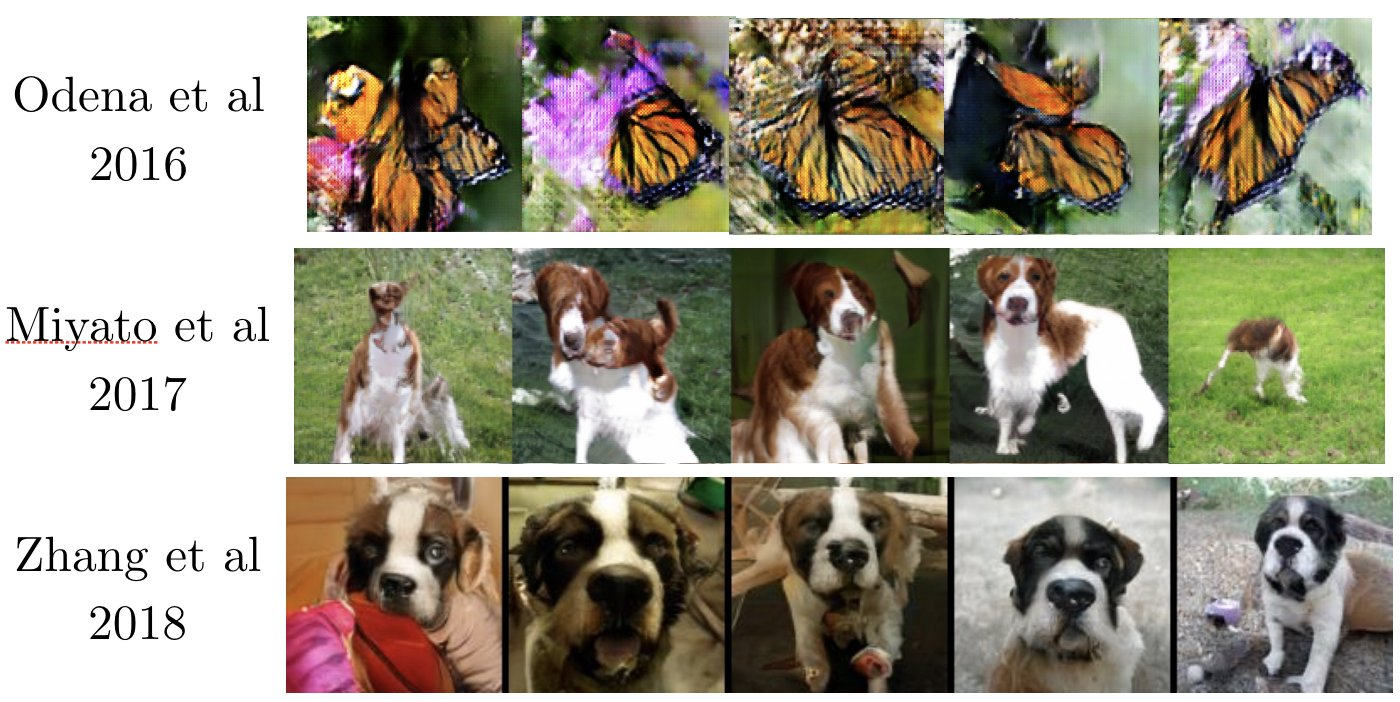
\includegraphics[width=0.8\textwidth]{images/gan_sota.jpeg}
\caption{2 года прогресса на датасете ImageNet-128~\cite{goodfellow_twi}}
\label{gan_sota}
\end{figure}

Тем не менее, такого же результата не удается добиться при генерации дискретных 
значений (как, например, текста). Причина кроется в природе 
генерируемых данных. Дело в том, что над непрерывными значениями гораздо проще 
определить всевозможные операции и преобразования, после чего эффективно 
оптимизировать функцию ошибки с помощью стохастического градиентного спуска. В 
дискретном же пространстве некоторые операции теряют свойство дифференцирования, 
из-за чего посчитать аналитически или программно производную по какой-либо 
переменной становится невозможным без специальных приемов, основанных на 
переходе к непрерывности. Помимо этого, сама структура текста 
предполагает некоторые сложности, связанные с долгосрочными зависимостями, 
омонимией и контекстом.

Существующие генеративные модели для текста обладают одним или нескольких 
недостатков:
\begin{itemize}
    \item Низкая связность или вариативность при генерации длинных примеров. Обычно, авторы ограничиваются наперед заданным ограничением длины в $10$-$15$ слов, которое хотелось бы расширить хотя бы вдвое.
    \item Невозможность эффективно использовать неразмеченные данные (которых бывает намного больше, чем данных с разметкой) при генерации с условием.
    \item Отсутствие интерпретируемости при формировании сэмпла.
\end{itemize}
В общем и целом, задача генерации текста остается нерешенной, или, по крайней
мере, решенной недостаточно хорошо, чтобы стать полезным инструментом для 
помощи человеку в реальных задачах.

Таким образом, целью данной работы является разработка генеративной модели, 
позволяющей производить эффективную, управляемую и интерпретируемую генерацию 
текстовых данных с увеличенной длиной в условиях данных с частичной разметкой, 
поддерживая связность, правдоподобие и разнообразие генерируемых примеров. 
Решение будет основываться на применении идей механизма внимания (attention) 
из глубокого обучения.

Постановка цели частично диктуется конкретными применениями в индустрии. 
Очень часто, входные данные обладают частично размеченными свойствами, набором
которых мы хотим параметризовать генерацию.
Например, мы хотим написать универсальный генератор текстовых условий задачек по 
заданным темам для онлайн курса по программированию, возможно облегчив работу 
авторам и составителям. Также, одно из возможных применений - генерация 
молекулярных структур по входному представлению SMILES~\cite{wiki:smiles} в виде 
последовательности дискретных величин (эквивалентных словам) по заданными 
характеристикам.

Для достижения описанной выше цели необходимо решить следующие задачи:
\begin{itemize}
    \item Проанализировать предметную область и существующие модели. Обозначить основные проблемы и пути к их решению.
    \item Выбрать данные для обучения и тестирования. Разобраться с предобработкой "сырых" входных последовательностей.
    \item Выбрать метрики и способы для оценки результата.
    \item Придумать и реализовать способы, позволяющие эффективно справляться с существующими проблемами.
    \item Произвести сравнение подходов и анализ результатов.
\end{itemize}

В главе $1$ будут описаны формальная постановка задачи генерации текста и 
существующие подходы к ее решению, а также их недостатки и достоинства. В главе
$2$ происходит описание используемых данных. Глава $3$ посвящена способам 
оценки алгоритмов генерации, а также тому, как правильно представить и сравнить 
результаты работы генеративных моделей. В главе $4$ описаны наиболее удачные 
подходы, которые дали ощутимый прирост в качестве работы, и трудности, с 
которыми пришлось столкнуться в процессе реализации. В главе $5$ проводится 
анализ результатов.

\section{Обзор предметной области}
В этой главе будут описаны формальная постановка задачи генерации текста и 
существующие подходы к ее решению, а также их недостатки и достоинства.

\subsection{Формальная постановка задачи}
\newcommand{\Xtrain}{X_{\texttt{train}}}
\newcommand{\pdata}{p_{\texttt{data}}}
\newcommand{\pmodel}{p_{\texttt{model}}}
Определимся формальной с постановкой задачи. Любая генеративная задача может 
быть сформулирована следующим образом: необходимо реализовать алгоритм, 
принимающий на вход обучающее множество примеров $x \in 
\Xtrain$ из генеральной 
совокупности $X$, распределенных по некому сложному распределению $\pdata$, и 
строящий распределение $\pmodel$, приближающее реальное. 
Алгоритм может реализовывать $\pmodel$ как 
конструктивно, приближая $\pdata$ заранее знакомым простым распределением 
(Рис.~\ref{density_estimation}), так и неявно, ограничиваясь 
только способностью эффективно (по памяти и времени исполнения) сэмплировать 
(=генерировать) новые примеры (Рис.~\ref{density_samples}).

\begin{figure}[H]
\centering
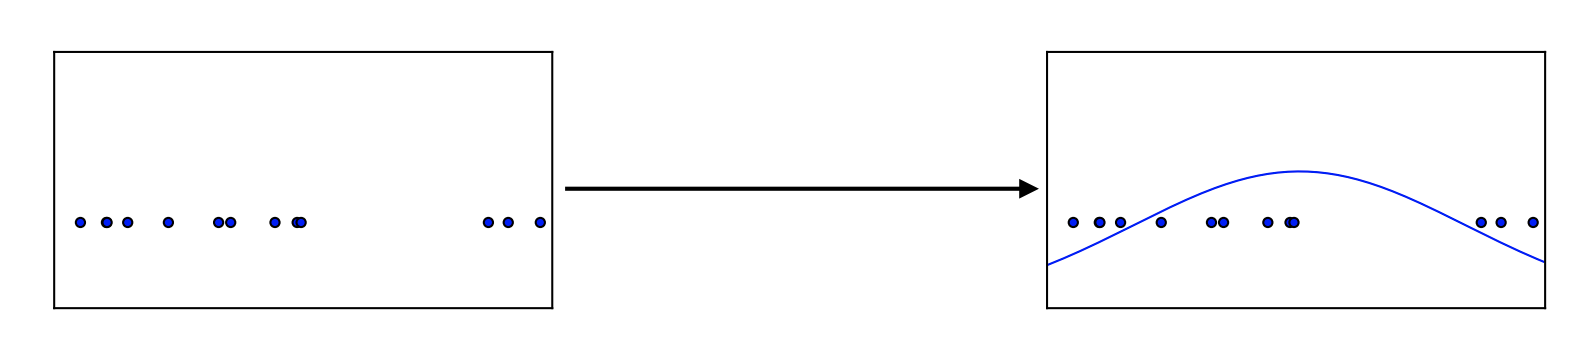
\includegraphics[width=\textwidth]{images/density_estimation.png}
\caption{Приближение $\pdata$ одномерной гаусианной~\cite{1701.00160}}
\label{density_estimation}
\end{figure}

\begin{figure}[H]
\centering
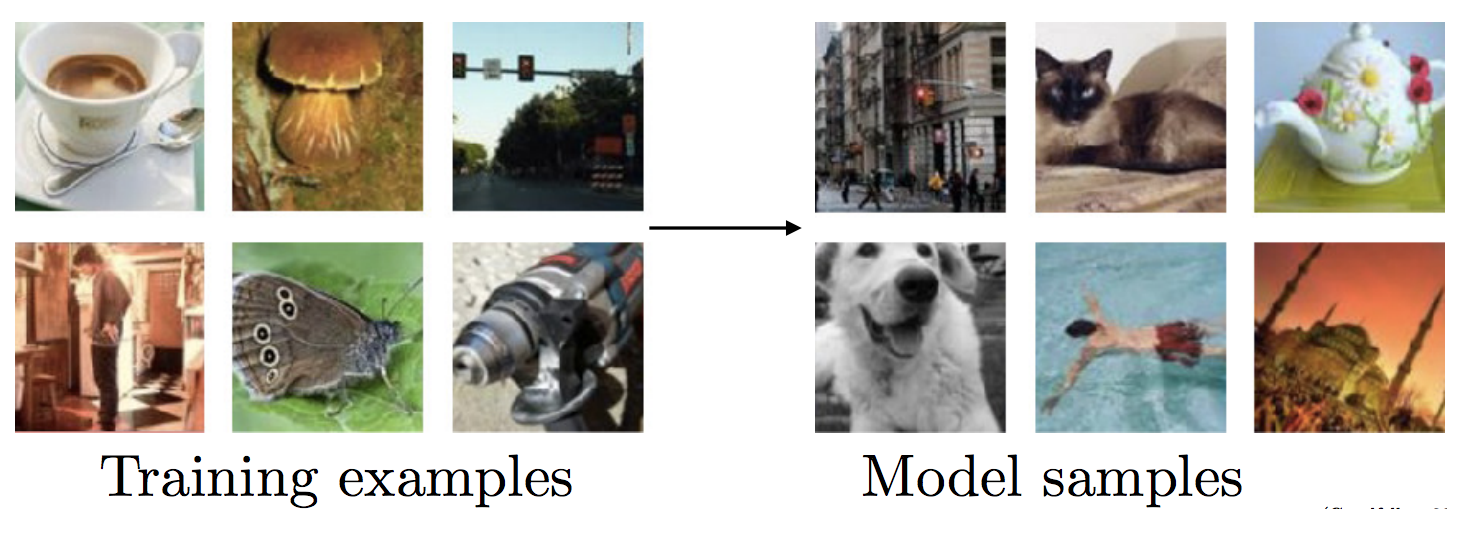
\includegraphics[width=0.85\textwidth]{images/density_samples.png}
\caption{Приближение $\pdata$ через сэмплирование новых примеров~\cite{1701.00160}}
\label{density_samples}
\end{figure}

В нашем случае, мы будем фокусироваться на проблеме генерации текстовых данных.
Обычно, они представлены в "сыром виде", то есть последовательностью
букв из конечного алфавита. Мы будем работать с английским языком, 
ввиду его распространенности, и, следовательно, простоты получения данных, хотя 
получившиеся модели не в коей мере не будут привязаны к конкретному языку и, 
более того, не будут привязаны к тексту вообще: мы можем считать данные 
последовательностями дискретных значений, о которых легче думать как о тексте.

Мы также расширим постановку задачи возможностью управляемой генерации и работы
с не размеченными данными. Признаки, присущие текстовой единице, это случайные 
величины $c$ (с априорным, обычно равномерным, распределением $p(c)$), 
конкретные значения которых могут представлять из себя категориальные 
или регрессионные свойства. Например, эмоциональная окраска (бинарное) или одна 
из $20$ предложенных тем. 
Такое расширение будет означать, что не все примеры из $\Xtrain$ могут быть 
размечены конкретными признаками, а сама генерация теперь может 
параметризовываться набором из свойств.

\subsection{Таксономия генеративных моделей}
В последнее время, все больше задач из машинного обучения успешно решаются с 
помощью подходов, основанных на нейронных сетях. В том числе, успешно удается
решать задачи из области обработки естественного языка, такие как суммаризация
текста, определение эмоциональной окраски и машинный перевод. Прорывной работой,
сместившей фокус внимания в области обработки естественного языка на нейронные
сети, можно считать работу~\cite{rnnlm}, которая успешно решала
задачу построения языковой модели с помощью рекуррентных нейронных сетей без
необходимости вручную или с помощью статистики улавливать закономерности и 
зависимости между словами в языке.

Предшествующие методы для генерации были либо 
основаны на правилах, либо на хорошо изученных вероятностных моделях, таких как
$n$-граммные модели или линейные модели~\cite{statmodel1, statmodel2}. 
Такие подходы,
несмотря на свою изученность и интерпретируемость, нуждаются в огромном 
количестве "ручной работы", в случае подходах, основанных на правилах, или 
просто имеют ограничение в качестве и точности работы, поэтому не могут 
эффективно использовать большие объемы данных \cite{1602.02410}. 
С другой стороны ставшие популярными в 
последние годы нейросетевые архитектуры, несмотря на хорошие результаты, плохо 
изучены и не всегда хорошо интерпретируемы. Несмотря на недостатки, в этой 
работе также будут использоваться нейронные модели с end2end архитектурами (то 
есть работающие напрямую с дискретными представлениями как на входе так 
и на выходе), в основном из-за своей эффективности и расширяемости.
Рисунок~\ref{approaches} иллюстрирует компромисс в сравнении работы двух 
подходов.

\begin{figure}[H]
\centering
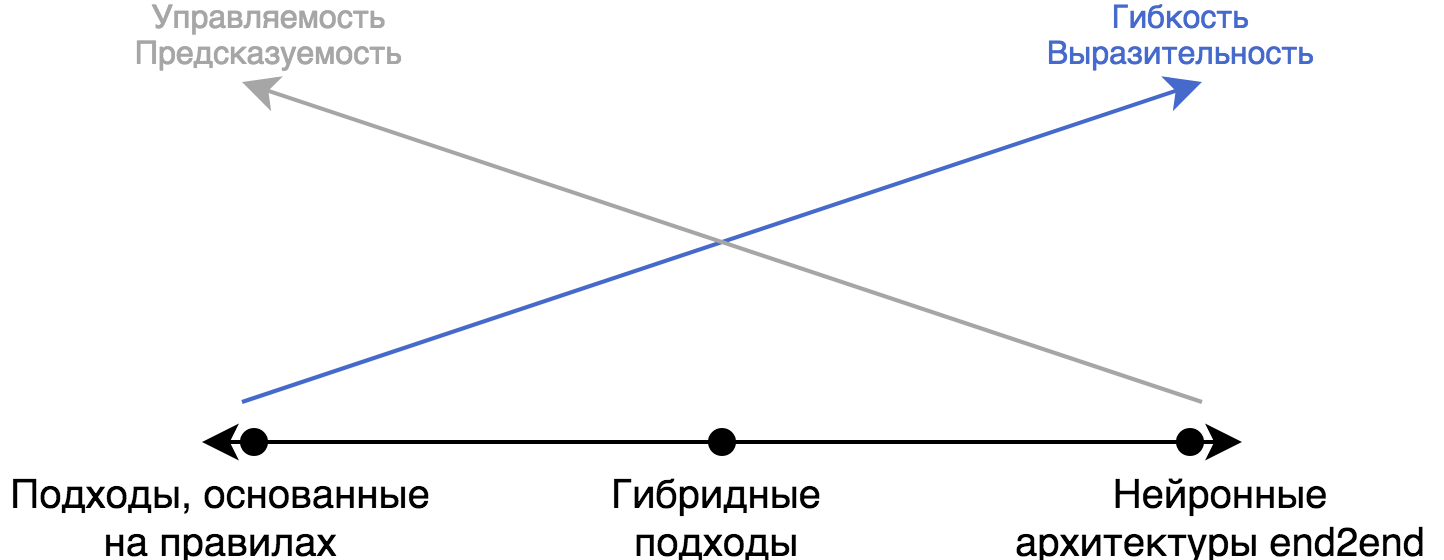
\includegraphics[width=0.9\textwidth]{images/approaches.png}
\caption{Сильные и слабые стороны подходов в обработке естественного языка}
\label{approaches}
\end{figure}

Процесс обучения нейросетевой архитектуры тесно связан с методом приближения 
истинного распределения $\pdata$. Большинство из них работают по 
\textbf{принципу максимального правдоподобия} (Рис.~\ref{mll_density}). Не 
все из них используют этот принцип напрямую, но могут быть переделаны или
переопределены так, чтобы так или иначе основываться на нем~\cite{1701.00160}.

\begin{figure}[H]
\centering
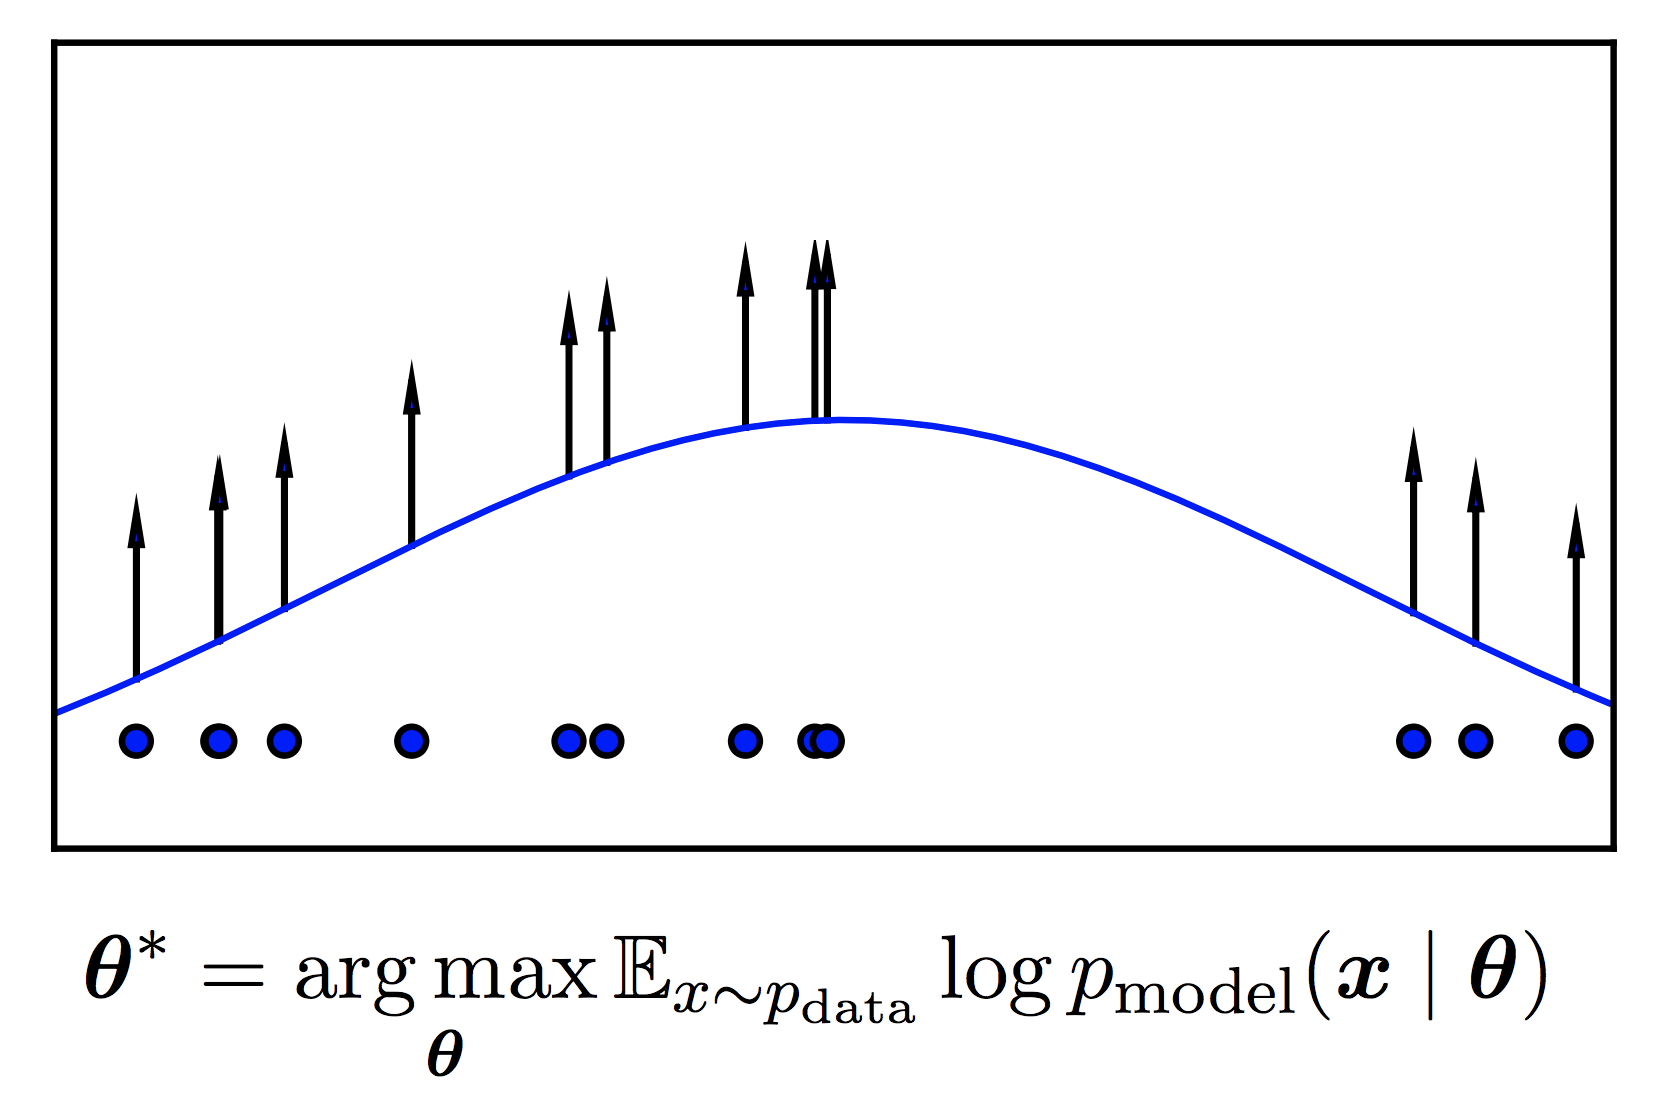
\includegraphics[width=0.7\textwidth]{images/mll_density.png}
\caption{Процесс обучения через принцип максимального правдоподобия~\cite{1701.00160}}
\label{mll_density}
\end{figure}

Нейронная архитектура моделирует распределение $\pmodel$, приближающее истинное
$\pdata$ и параметризованное набором весом $\theta$. Сам принцип максимально 
правдоподобия есть ни что иное, как выбор параметров модели, максимизирующих
правдоподобие тренировочных данных по Формуле~\ref{log_maximum_likelihood}. 
Легче всего это производится в $\log$-пространстве, так как мы заменяем 
произведение по тренировочным примерам на сумму. Сумма
упрощает численную реализацию и подсчет градиента, а также 
позволяет избежать проблем с переполнением чисел с плавающей точкой. 

\begin{equation}
\label{log_maximum_likelihood}
\begin{split}
\theta^* = \argmax_{\theta} \prod^{n}_{i=1}{\pmodel(x^{(i)}; \theta)} \\
= \argmax_{\theta} \log \prod^{n}_{i=1}{\pmodel(x^{(i)}; \theta)} \\
= \argmax_{\theta} \sum\limits^{n}_{i=1}{\log \pmodel(x^{(i)}; \theta)}
\end{split}
\end{equation}

Максимизация правдоподобия может быть рассмотрена как эквивалентная минимизации
дивергеции Кульбака-Лейблера~\cite{wiki:kldiv}, которая задает
расстояние между распределениями. Точнее, если бы нам удалось точно приблизить 
$\pdata$, то оно бы принадлежало семейству распределений $\pmodel(x; \theta)$. 
На практике мы не имеем доступа к $\pdata$, а лишь знаем о $n$ точках из 
тренировочной выборки, которые мы используем чтобы задать $\hat 
p_{\texttt{data}}$ - эмпирическое распределение, аппроксимирующее $\pdata$. 
Минимизация дивергеции Кульбака-Лейблера между $\hat p_{\texttt{data}}$ и 
$\pmodel$ в точности эквивалентна максимизации правдоподобия
(Формула~\ref{kl_maximum_likelihood}).

\begin{equation}
\label{kl_maximum_likelihood}
\theta^* = \argmin_{\theta} D_{KL}(\hat p_{\texttt{data}}(x) || \pmodel(x; \theta))
\end{equation}

Если мы сузим внимание на глубокие нейросетевые архитектуры, основанные на 
вариациях метода максимизации правдоподобия, то можем ввести некую таксономию 
на разнообразие генеративных моделей в зависимости от того, как именно 
приближается исходное распределение (Рис.~\ref{gen_taxonomy2}). Каждый лист в
дереве на рисунке соответствует конкретному классу моделей, имеющему свои 
достоинства и недостатки. Нас не будут интересовать модели, основанные на 
марковских цепях, так как они имеют некоторые проблемы с стоимостью получения и 
корреляцией между сэмплами~\cite{vetrovgan}. Далее, мы 
последовательно рассмотрим модели с возможностью явно выразить распределение 
(RNN), модели с аппроксимаций распределения (VAE) и неявные вероятностные 
модели (GAN). Более точно, нас будут интересовать вариации этих подходов для 
задач генерации текста.

\begin{figure}[H]
\centering
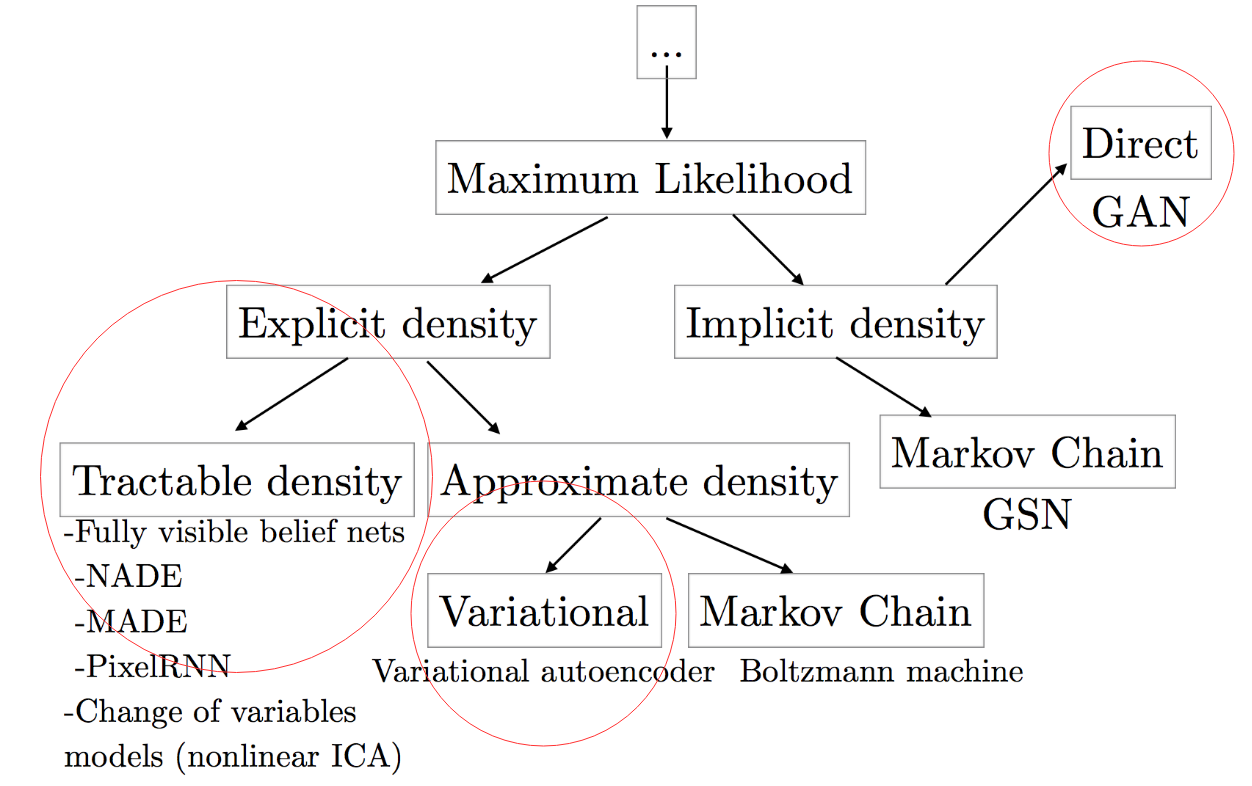
\includegraphics[width=\textwidth]{images/gen_taxonomy2.png}
\caption{Таксономия генеративных моделей~\cite{1701.00160}}
\label{gen_taxonomy2}
\end{figure}

\subsection{RNN}
Рекуррентные нейронные сети - базовая модель, использующая принцип максимального 
правдоподобия напрямую.

\subsubsection{Обучение}
На вход для обучения сети поступает набор из последовательностей 
$x = (x_1, \cdots, x_{|x|})$. $x_i$ - числовые представление слов из словаря,
фиксированного размера, закодированные 
после токенизации~\cite{wiki:token} "сырой" входной последовательности. Стоит
также отметить, что получившиеся слова не всегда соответствуют словам в 
привычном понимании (из естественного языка): они также могут быть любым другим
однозначным разбиением последовательности из символов - например, кусками из BPE
разбиения или вовсе обычными одиночными символам~\cite{1508.07909, charnn}. Мы 
хотим смоделировать совместную вероятность слов по формуле \ref{rnn_density}, 
что в свою очередь эквивалентно формуле \ref{log_rnn_density} при переходе в 
$\log$-пространство.

\begin{equation}
\label{rnn_density}
p(x) = \prod^{|x|}_{i=1}{p(x_i | p_{<i})}
\end{equation}

\begin{equation}
\label{log_rnn_density}
\log p(x) = \sum\limits^{|x|}_{i=1}{\log p(x_i | p_{<i})}
\end{equation}

Архитектура RNN представлена на рисунке $\ref{rnn_unrolled}$. RNN - это 
последовательность из $|x|$ шагов нелинейных преобразований, принимающих 
очередную часть $x_i$ и скрытое представление $h_{i-1}$ c прошлого шага. Так как
изначально $x_i$ находятся в дискретном поле, перед скармливанию сети $x_i$ 
обычное векторизуют (переводят в непрерывное пространство). Для векторизации 
могут использоваться как обычное one-hot представление~\cite{onehot}, имеющее
смысл лишь при маленьком размере словаря, так более продвинутые векторные 
представления слов с семантической нагрузкой~\cite{word2vec, glove, elmo}. 
Преобразования $A$, параметризованные неким набором весов (параметров), 
сохраняют непрерывность и возможность посчитать градиент, 
а сам тип преобразования зависит от вида рекуррентной сети.
Обычно используются популярные в последнее 
время и наиболее удачны архитектурно, \textbf{GRU}~\cite{1412.3555} и 
\textbf{LSTM}~\cite{lstm}, эффективно борящиеся с проблемой затухающих 
градиентов на длинных последовательностях.

\begin{figure}[H]
\centering
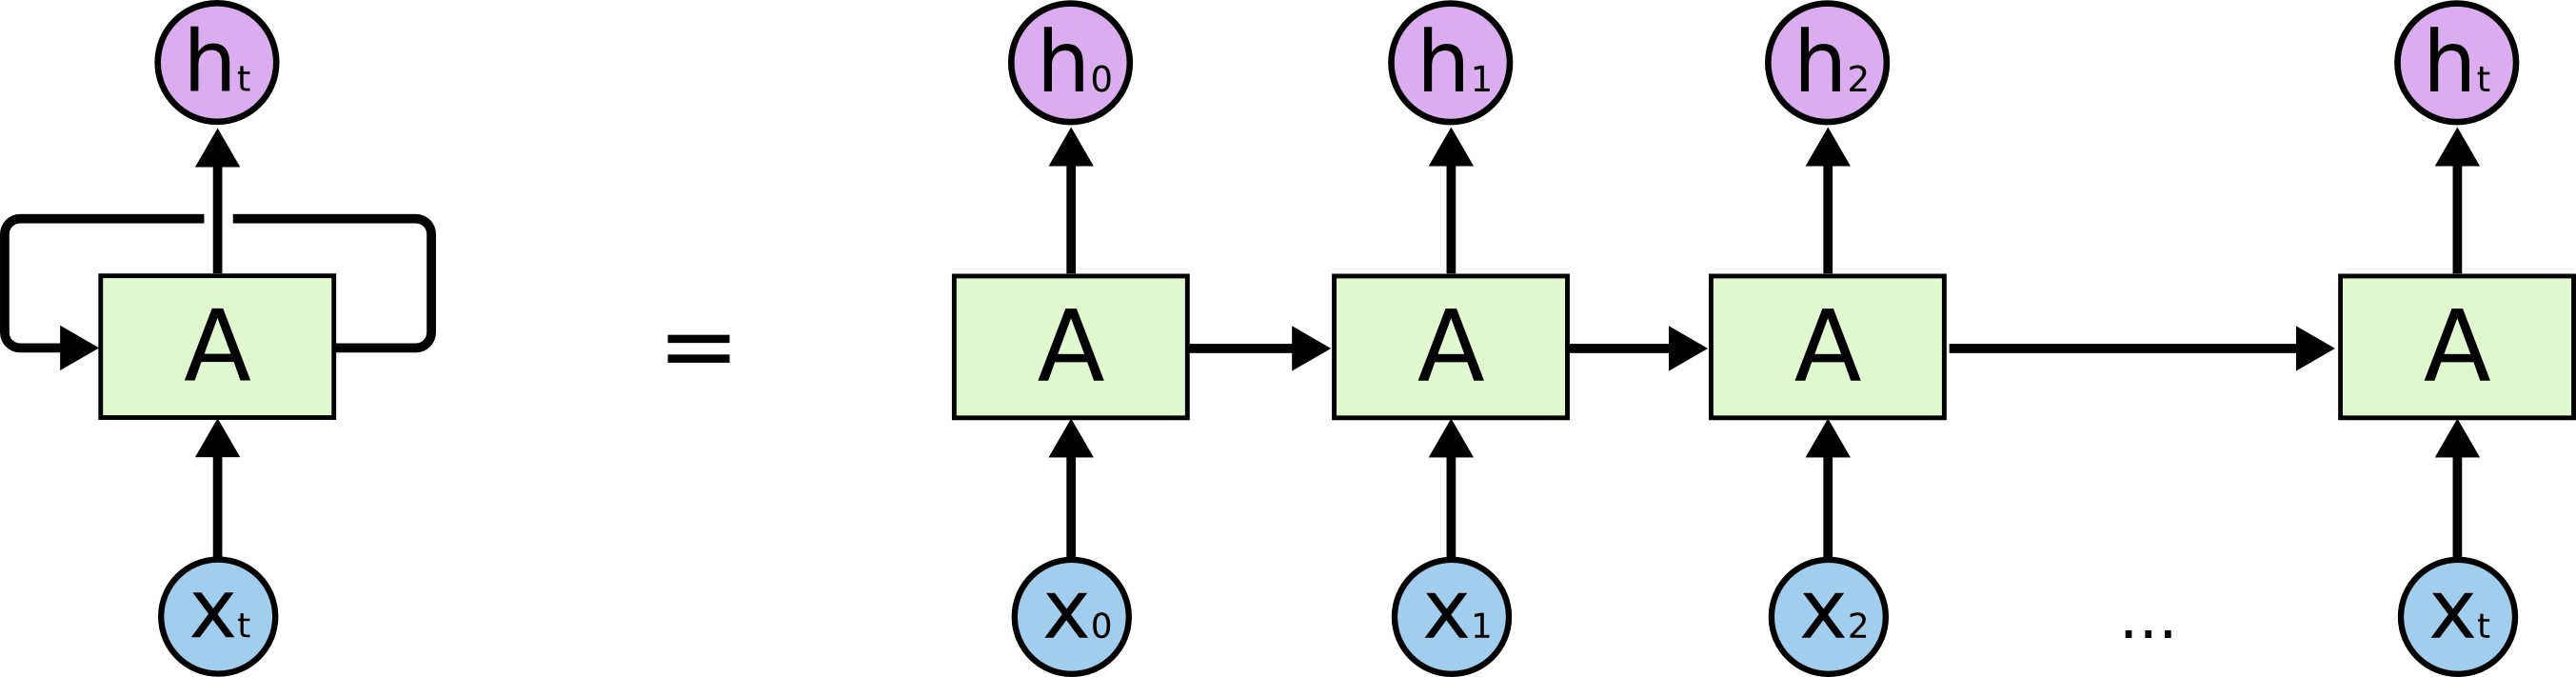
\includegraphics[width=\textwidth]{images/rnn_unrolled.png}
\caption{Схема работы рекуррентной нейронной сети~\cite{medium:rnn}}
\label{rnn_unrolled}
\end{figure}

Для того, чтобы посчитать $p(x_i|x_{<i})$ на очередном шаге RNN, используется 
очередное скрытое представление $h_i$. Например, мы можем применить полносвязный
слой~\cite{cnn}, переводящий $h_i$ в вектор $\mathbb{R}^{|V|}$, далее применить 
софтмакс активацию~\cite{wiki:softmax}, после которой мы фактически получаем 
распределение на вероятность следующего слова из словаря. 
Такое распределение можно 
противопоставить "истинному распределению", то есть one-hot представлению 
нужного символа, который известен в процессе обучения. 
Далее, мы можем выразить некое 
расстояние между распределениями, например, кросс-энтропию или дивергенцию 
Кульбака-Лейблера (их минимизация эквивалентна друг-другу). Итоговая ошибка - 
сумма ошибок на каждом шаге. Оптимизация происходит, обыкновенно, какой-либо 
вариацией стохастического градиентного спуска~\cite{optimizers} с обрезанием 
значений вектора градиента~\cite{gradient_clipping}.

\subsubsection{Генерация}
Теперь опишем подробно, как происходит генерация. Здесь мы будем 
подразумевать генерацию случайных сэмплов без предусловия, а механизмы 
расширений для условной генерации будут описаны далее.

\newcommand{\bos}{\langle bos \rangle}
\newcommand{\sos}{\langle sos \rangle}
\newcommand{\eos}{\langle eos \rangle}
\newcommand{\unk}{\langle unk \rangle}
\newcommand{\pad}{\langle pad \rangle}
Обычно, полагается, что любой $x$ из данных для обучения - цельный, законченный 
отрывок текста из пары предложений, обрамленный с начала и конца соответственно 
условными словам $\bos/\sos$ и $\eos$ - символами начали и конца (begin of 
sequence, start of sequence, end of sequence). Для того, чтобы начать генерацию, 
мы подаем нашей модели на вход символ начала, а заканчиваем процесс, когда 
встретили символ конца (или достигли наперед заданного ограничения в 
максимальную длину сэмпла).

Как мы уже выяснили, RNN задает явное распределение $p(x_i|x_{<i})$ на очередном
шаге генерации. Самый очевидный и не совсем удачный способ - просэмплировать
очередной $x_i$ и двинуться дальше. Еще более плохой путь - взять 
$\argmax p(x_i|x_{<i})$ (несложно понять, что так мы всегда будем 
генерировать ровно один уникальный пример). О дихотомии этих двух крайностей и 
о более удачных подходах будет описано подробнее в главе $4$. В общем же 
случае, процесс генерации, это хождение по дереву возможных вариантов
(Рис.~\ref{beam_search}). Нас будут интересовать пути с наибольшей совместной 
вероятностью слов. Несложно понять, что задача поиска таких путей NP-трудна и 
без перебора эффективно решить ее не получится. Также стоит отметить, что в 
идеале нам надо искать сразу $k > 1$ наиболее правдоподобных примеров для 
повышения разнообразия генеративной модели.

\begin{figure}[H]
\centering
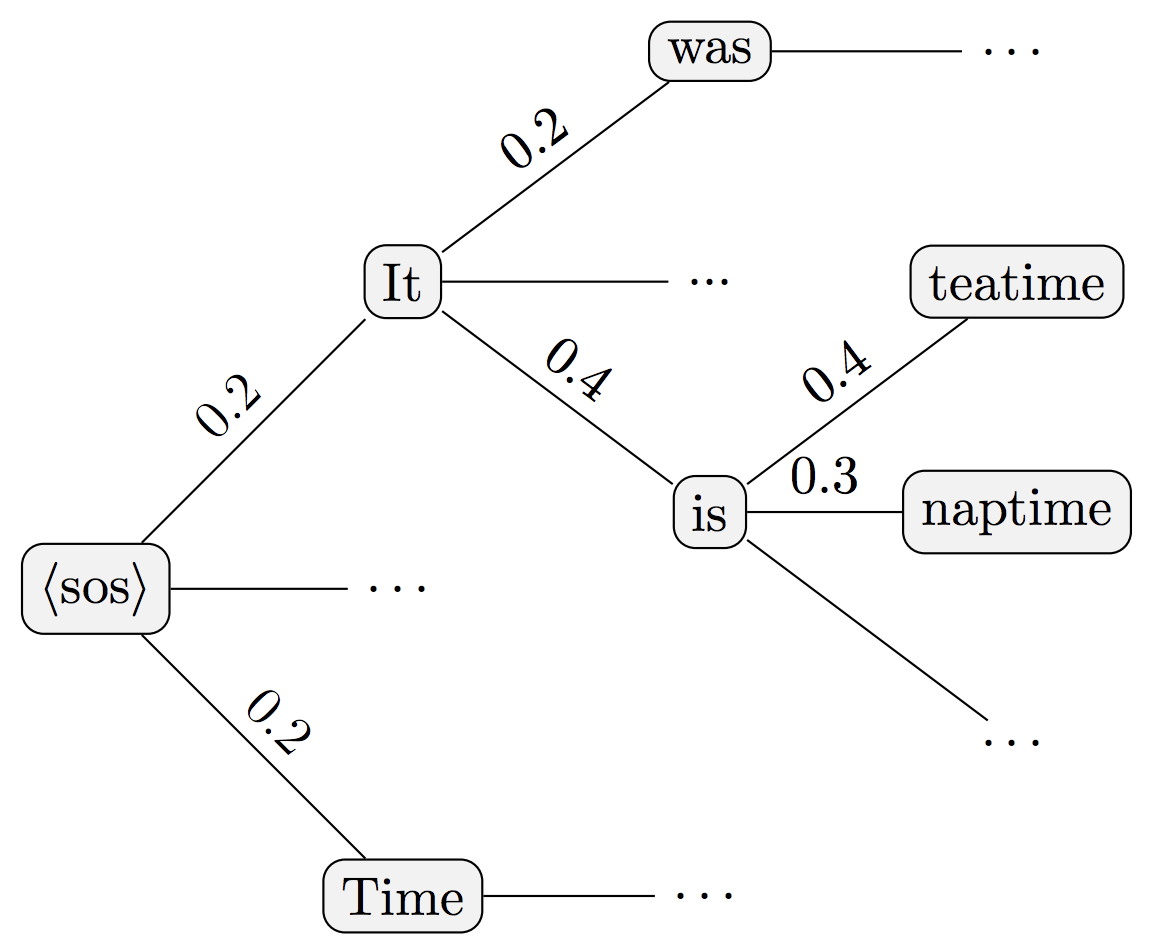
\includegraphics[width=0.6\textwidth]{images/beam_search.png}
\caption{Процесс генерации в виде хождения по дереву}
\label{beam_search}
\end{figure}

\subsubsection{Преимущества и недостатки}
RNN - базовая модель, так или иначе использующаяся во всех подходах к генерации
строк. Она обладает целым набором преимуществ, но и сильных недостатков, не
позволяющих использовать ее для нашей задачи.

К достоинствам можно отнести:
\begin{itemize}
    \item Эффективное и простое обучение: одна ошибка, один градиент, целый 
    набор приемов по оптимизации.
    \item Расширяемая и простая реализация. RNN - базовая модель, поэтому она
    часть берется за основу и расширяется в сторону увеличения скорости 
    тренировки, предотвращения переобучения, повышения интерпретируемости и 
    глубины. К известным методам~\cite{bengio_rnn} можно отнести: 
    multi-layer rnn, bidirectional rnn~\cite{bidir_rnn}, 
    dropout~\cite{wiki:dropout}, scheduled sampling~\cite{1506.03099},
    attention~\cite{attention_rnn}, ensembling~\cite{wiki:ensebling},
    hierachy~\cite{1609.01704}, sru~\cite{1709.02755} и некоторые другие.
    \item Эффективное сэмплирование. Стоимость получения сэмпла низкая, возможно
    оценить совместную вероятность для подсчета метрик (Формула~\ref{perplexity}),
    а также расширить алгоритм генерации эвристиками и регуляризацией.
\end{itemize}

К недостаткам относятся:
\begin{itemize}
    \item Небольшая эффективность по метрикам и быстрая потеря связности 
    начала с концом. Bengio~\cite{bengio_rnn}, к примеру, связывает это с 
    отсутствием изначального представления генерируемого сэмпла. Мы 
    начинаем генерацию из пустоты, на ходу, слово за словом пытаясь создавать
    правдоподобный экземпляр, что приводит к плохой связности (coherence) при
    генерации.
    \item RNN работает только в условиях полной разметки данных. Если же данные
    размечены плохо или на части данных отсутствует разметка вовсе, то учесть
    это в стандартной рекуррентной нейронной сети - нетривиальная задача.
    \item Управляемая генерация. Чтобы задать начальные условия для генерации в 
    RNN, можно конкатенировать параметры условия с входом 
    $x_i$ на каждом шаге генерации (out-of-band) или добавить свойства текста
    в сам текст в качестве префикса и суффикса, тогда можно начинать генерацию
    с нужного префикса (in-band). Оба эти подхода работают плохо даже на самых
    простых данных~\cite{rnn_meta}.
\end{itemize}

В общем и целом, RNN - хорошая базовая модель, недостатки которой пытаются 
преодолеть в других подходах.

\subsection{VAE}
Одна из популярных архитектур генеративных моделей - вариационные автоэнкодеры
(variational autoencoder, VAE). VAE основаны на вариационном продолжении 
автоэнкодеров, выучивающих латентное представление обучающих примеров.

\subsubsection{Обзор}
Архитектура автоэнкодеров представляет из себя $2$ нейронные сетки - энкодер, 
переводящий сэмпл $x \in \mathbb{R}^n$ в латентное представление 
$z \in \mathbb{R}^m,~m \ll n$, и декодер, моделирующий обратное преобразование. 
Ошибка сети есть ошибка восстановления на батчах из тренировочного набора. AE -
модель обучения без учителя, позволяющая сжать входные данные до пространства
меньшего размера, получив универсальный трансформатор $x$ в латентное 
представление $z$. $z$ может быть в дальнейшем использоваться в том числе и для
обучения с учителем.

Декодер в архитектуре АЕ фактически представляет из себя этакий генератор $x$
по заданному латентному представлению. Однако, полноценно использовать его для
задач генерации не получится. В обычном AE мы не моделируем $\pmodel$, 
приближающее $\pdata$, поэтому и непонятно откуда сэмплировать $z$, чтобы 
генерировать новые примеры. 

VAE решает эту проблему. Пусть $x$ как и $z$ - случайные величины, имеющие
распределения $\pdata$ и $p(z) = N(0, I)$ соответственно. Выбор гаусианы в 
качестве априорного не случаен - это простое распределение, с которым гораздо 
легче решать задачу оптимизации. 
Скажем теперь, что энкодер $q(z|x)$ будет аппроксимировать сложное 
апостериорное распределение $p(z|x)$ и также будет делать это многомерной
гаусианой, сразу предсказывая среднее и дисперсию по каждой компоненте. Декодер
же будет отвечать за восстановление $x \sim p_{\theta}(x|z)$ 
(Рис.~\ref{vae_terms}). 

\begin{figure}[H]
\centering
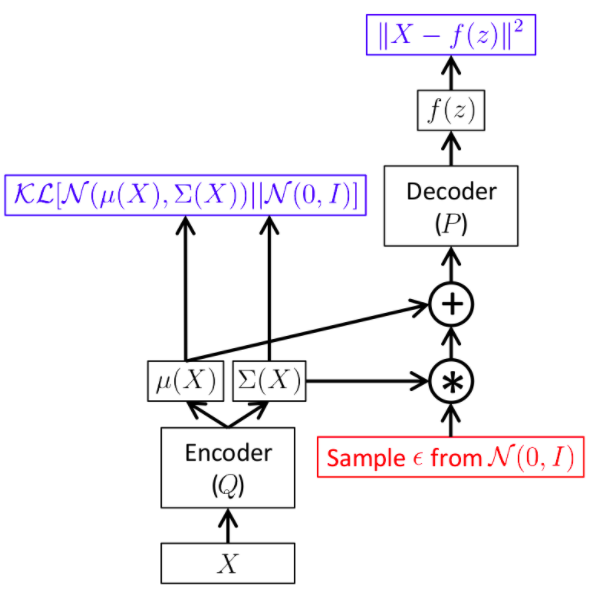
\includegraphics[width=0.5\textwidth]{images/vae_terms.png}
\caption{Архитектура VAE~\cite{habr:vae}}
\label{vae_terms}
\end{figure}

Попытаемся выписать логарифм правдоподобия на тренировочном наборе. Известный 
результат - нижняя вариационная оценка ELBO~\cite{vae} - представлена на 
Формуле~\ref{elbo}. Фактически, мы зажимаем правдоподобие снизу формулой, 
которую можно оптимизировать напрямую по весам энкодера и декодера. 
Второй терм - дивергенция Кульбака-Лейблера между двумя гаусианами - имеет 
аналитическое решение и может быть выражена с помощью дифференцируемых 
преобразований. 
Тонкий момент - пробрасывание градиента через сэмплирование из апостериорного 
распределения $q$. Его можно избежать если заранее просэмплировать значения из
белого шума, а потом параметризовать его предсказанными матожиданием и 
дисперсией (Рис.~\ref{vae_terms}).

\begin{equation}
\label{elbo}
\log p(x) \geqslant \mathbb{E}_z{[\log p_{\theta}(x|z)]} - D_{KL}{(q(z|x) || p(z))}
\end{equation}

Итак, ошибка у VAE - сумма ошибки восстановления по аналогии с AE и kl-терм, 
выражающий расстояние между двумя гаусианами - аппроксимацией апостериорного и
априорным распределениями. В данном случае kl-терм можно интерепретировать как 
регуляризацию на форму латентного пространства.

Теперь мы получаем возможность сэмплировать из $\pmodel$. 
Возьмем $z \sim p(z)$ и передадим в декодер 
$p_{\theta}{(x|z)}$. Получили эффективный, низкий по стоимости и легкий в 
обучении генератор сэмплов, то есть генеративную модель.

\subsubsection{Дискретные данные}
Впервые, успешно применить VAE для генерации дискретных значений удалось 
Bowman et al.~\cite{text_vae}. Энкодер и декодер представляют из себя 
рекуррентные нейронные сети LSTM, энкодер с последнего слоя с последнего 
скрытого представления генерирует матожидание и дисперсию для апостериорного
распределения, а к декодеру на каждый входной $x$ добавляется скрытый вектор
$z$. Схематически архитектура изображена на Рисунке~\ref{text_vae}.

\begin{figure}[H]
\centering
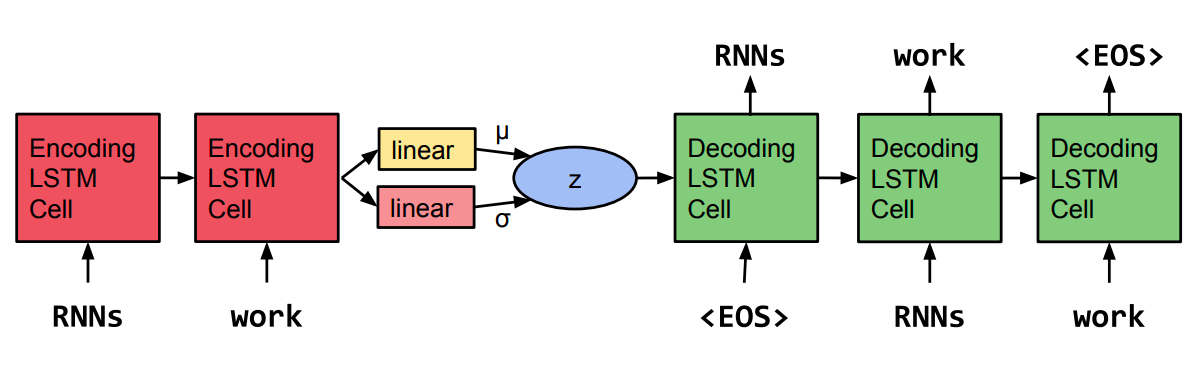
\includegraphics[width=\textwidth]{images/text_vae.png}
\caption{Архитектура TextVAE~\cite{text_vae}}
\label{text_vae}
\end{figure}

Несмотря на простоту подхода, такой вариант реализации не будет работать 
правильно. Дело в том, что декодер начинает учиться намного быстрее энкодера,
поэтому сеть игнорирует часть ошибку с kl-термом. 
Чтобы этого избежать, вес у kl части 
ошибки следует постепенно прибавлять по какой-нибудь гладкой функции от $0$ 
до $1$ (Рис.~\ref{kl_term_w}). Мы также будем немного портить жизнь декодеру, 
применяя вместо обычного новый "word dropout" - в процессе обучения случайно 
заменяя последнее слово на $\unk$.

\begin{figure}[H]
\centering
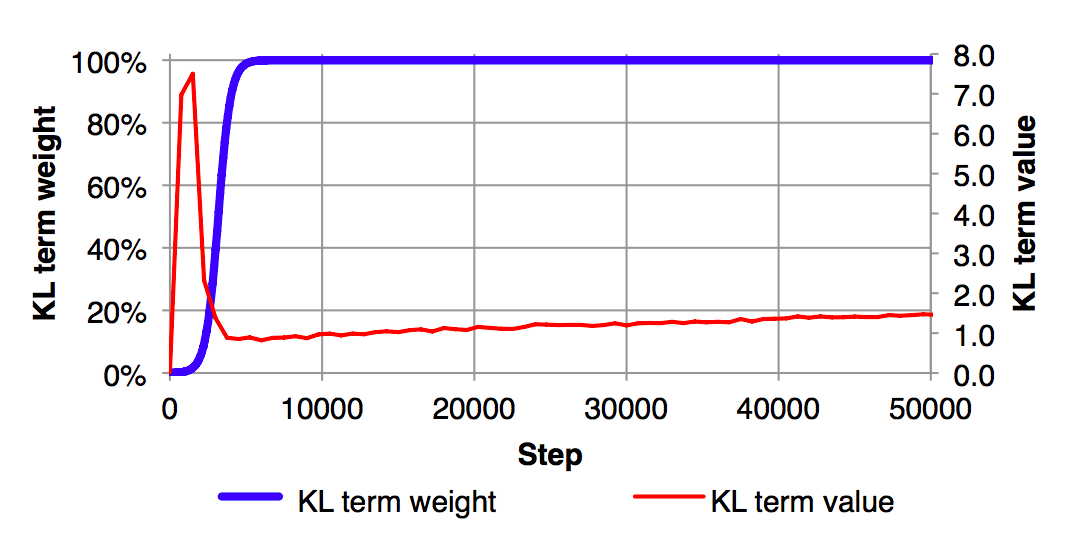
\includegraphics[width=0.85\textwidth]{images/kl_term_w.png}
\caption{Изменение kl-терма в процессе обучения~\cite{text_vae}}
\label{kl_term_w}
\end{figure}

Теперь TextVAE можно успешно обучить, получив интересные интерпретируемые 
свойства. Семантический смысл, относительно латентного 
пространства, начинает плавно перетекать от предложения к предложению. Чтобы 
заметить это, давайте возьмем две точки в латентном пространстве и начнем 
декодировать $z$ на пути от одной до другой. Видно, что для AE 
(Рис.~\ref{ae_path}) переход не плавный, а для VAE (Рис.~\ref{vae_path}) любые 
два соседа на пути семантически близки.

\begin{figure}[H]
\centering
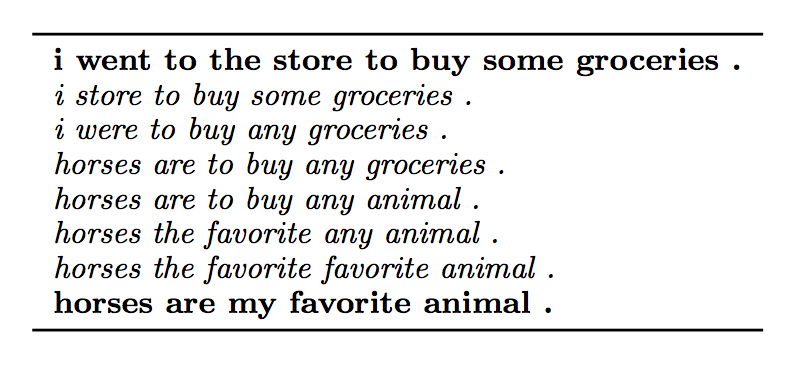
\includegraphics[width=0.7\textwidth]{images/ae_path.png}
\caption{Декодированный путь между точками в латентном пространстве для AE~\cite{text_vae}}
\label{ae_path}
\end{figure}

\begin{figure}[H]
\centering
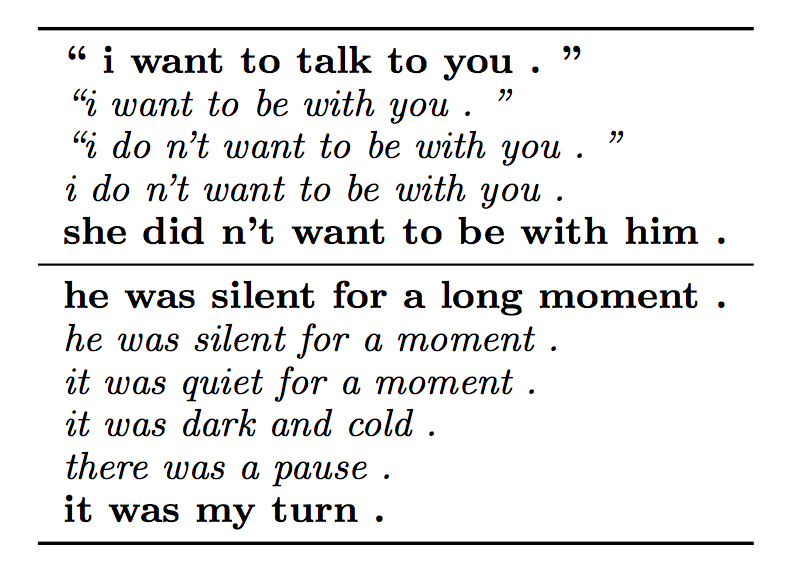
\includegraphics[width=0.6\textwidth]{images/vae_path.png}
\caption{Декодированный путь между точками в латентном пространстве для VAE~\cite{text_vae}}
\label{vae_path}
\end{figure}

Оригинальная модель Text VAE не подходит для набора данных с частичной разметкой, 
а также не поддерживает условную генерацию. Расширение для таких задач было 
предложено в~\cite{text_cvae}. Архитектура изображена на 
Рисунке~\ref{cvae}. К латентному пространству добавился независимый код $c$,
отвечающий за контролируемое свойство в данных. Декодер разделился на генератор 
и дискриминатор, отвечающий соответствие свойств и данных. Фактически, 
дискриминатор это классификатор в случае категориального свойства и регрессор в
случае непрерывного. Мы больше не сможем оптимизировать всю модель, задав общую
ошибку, из-за того, что дискриминатор принимает дискретное $x$, полученное от
генератора. Процесс оптимизации происходит итеративно в цикле: сначала мы 
делаем шаг по весам дискриминатора, а потом шаг по весам VAE (энкодер + 
генератор). Для того, чтобы избежать проблемы расхождения в качестве генератора
и дискриминатора, на вход для оптимизации последнему подается также 
"soft sample" - матожидание для сэмпла генератора без необходимости
реально сэмплировать из дискретного распределения, а значит без потери свойства
непрерывности и возможности посчитать градиент.

\begin{figure}[H]
\centering
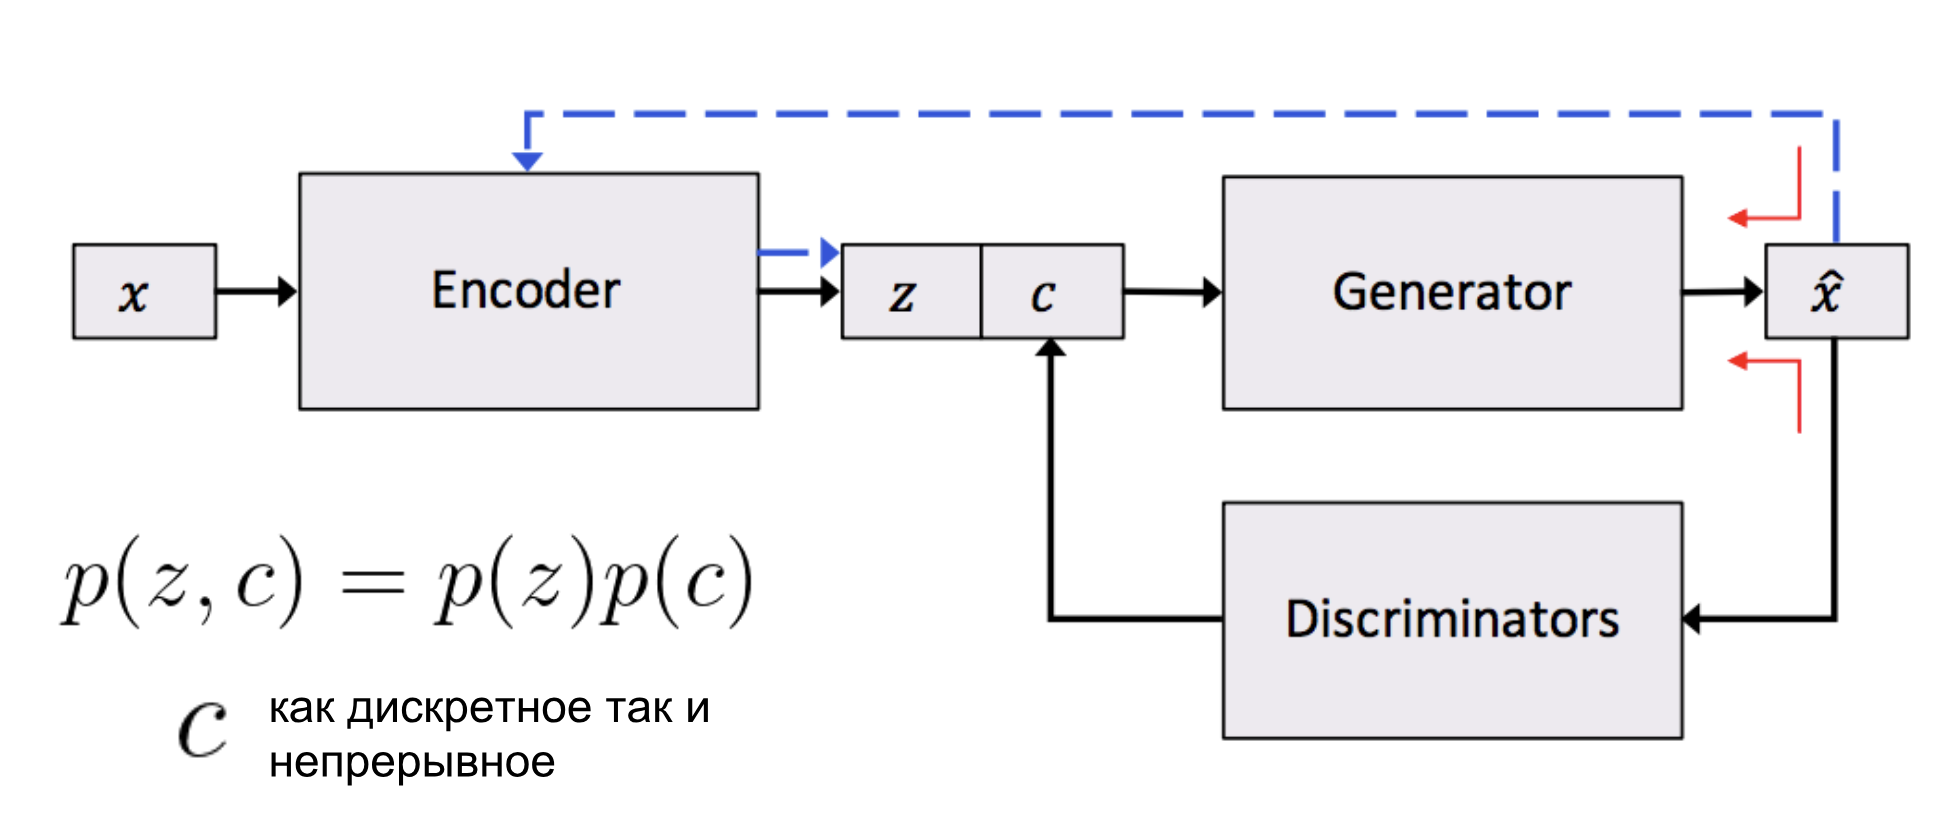
\includegraphics[width=0.7\textwidth]{images/cvae.png}
\caption{Архитектура Conditional TextVAE~\cite{text_cvae}}
\label{cvae}
\end{figure}

В общем и целом, Conditional TextVAE удовлетворяет всем вышеперечисленным 
требованиям. Во-первых, нам не обязательно иметь разметку свойств на всех 
данных: при отсутствие $c$ мы можем просэмплировать его из априорного $p(c)$ в
процессе оптимизации. Во-вторых, количество свойств не ограничено одним: на 
каждый тип $c$ мы можем тренировать свой дискриминатор. В-третьих, теперь мы
можем полностью контролировать процесс генерации, задав нужные $c$ (или взяв
их из априорных) и передав генератору. Тесты показывают, что Conditional TextVAE
требуется совсем немного примеров, чтобы эффективно параметризовать генерацию
управляемыми свойствами \cite{text_cvae}. Проблемы TextVAE это медленная
оптимизация и ограничения в длине генерируемого сэмпла. Авторы оригинальной 
статьи ограничились длинной в $15$ слов, теряя связность при генерации более
длинных $x$.

\subsection{GAN}
Класс моделей, показывающих лучшие результаты в задачах генерации - 
генеративно-состязательные сети (generative adversarial networks, GAN). В этой 
части, мы кратко рассмотрим принцип работы и расширения для генерации дискретных 
значений.

\subsubsection{Обзор}
Основная идея GAN~\cite{1406.2661} - переформулировка задачи в терминах 
игры с нулевой суммой между двумя игроками-сетями, генератором и 
дискриминатором. Генератор отвечает за непосредственно низкую по стоимости 
генерацию новых примеров по распределению $\pmodel$, принимая на вход случайных 
шум. Дискриминатор же - это классификатор, пытающийся по $x$ определить,
пришел ли он из $\pmodel$ или из $\pdata$. Генератор обучается, чтобы обманывать 
дискриминатор, а дискриминатор, наоборот, не давать генератору обмануть себя. 
Процесс показан на Рисунке~\ref{gan_fw}.

\begin{figure}[H]
\centering
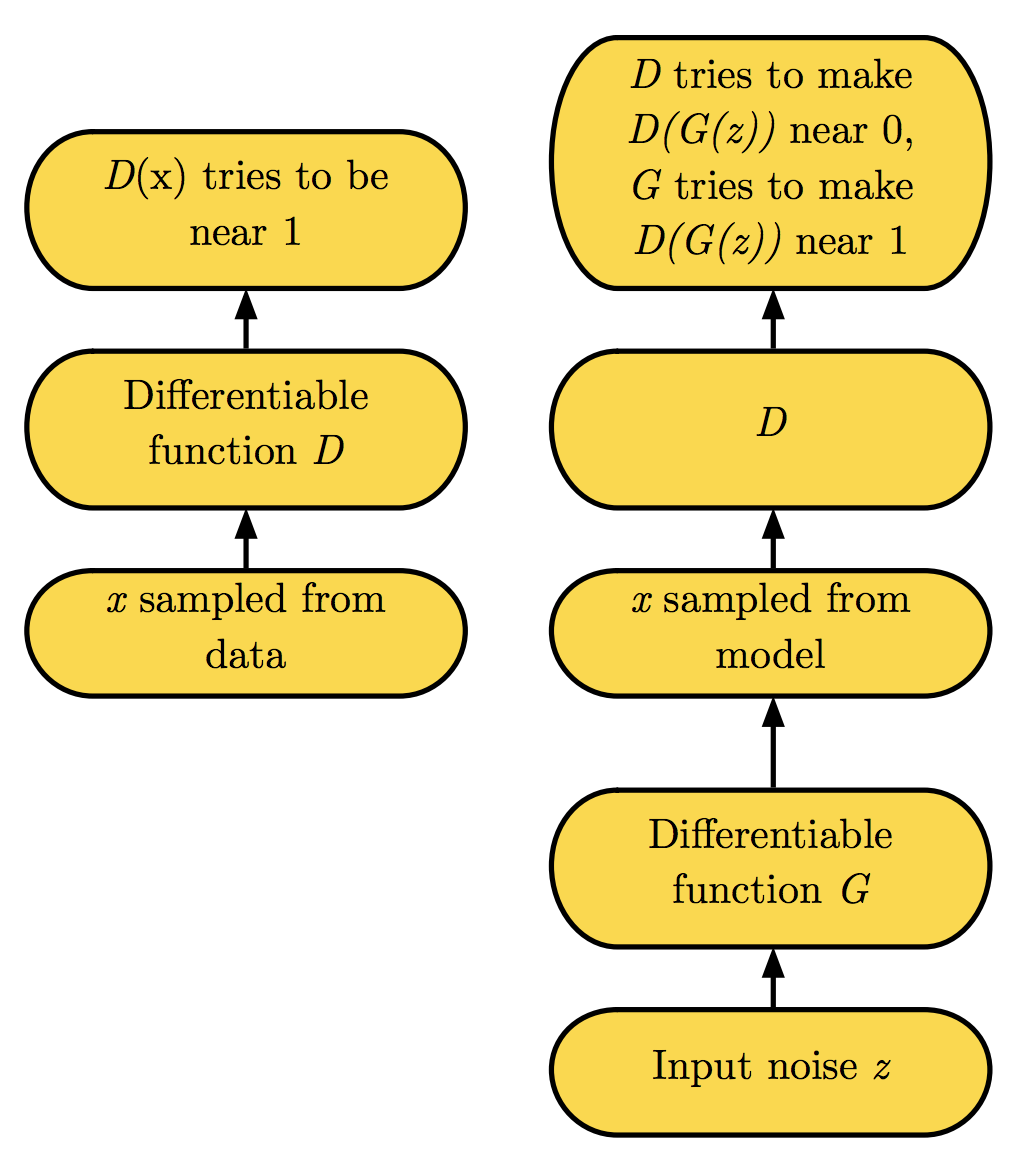
\includegraphics[width=0.5\textwidth]{images/gan_fw.png}
\caption{Архитектура GAN~\cite{1701.00160}}
\label{gan_fw}
\end{figure}

Два игрока представлены двумя нейронными сетями, каждая из которых 
дифференцируема по входным аргументам и по своим весам. Дискриминатор принимает
на вход $x$ и параметризован $\theta^{(D)}$. Генератор принимает на вход 
латентный вектор $z$, просэмплированный из некого априорного
распределения, и параметризован $\theta^{(G)}$. Каждый из игроков имеет свою
функцию ошибки, которая зависит от аргументов - весов собственной сетки. Так как
каждый из игроков не имеет доступа к параметрам другого и может изменять 
собственное поведение с помощью своих параметров, сценарий более 
естественно определить как игру, нежели как задачу оптимизации. Решение такой
игры - это равновесия Нэша - набор из $\theta^{(D)}$ и $\theta^{(G)}$, так что
каждая из функций ошибок находится в локальном минимуме по своим весам.

Тренировочный процесс в GAN это процесс из одновременных стохастических 
градиентных спусков. На каждом шаге, мы сэмплируем два батча данных: один из
тренировочной выборки $x \sim \pdata$, один из генератора $x \sim \pmodel$. 
Далее, мы делаем два шага оптимизации: один по весам $\theta^{(D)}$, другой 
по весам $\theta^{(G)}$. Некоторые работы советуют делать разное количество 
шагов у генератора и дискриминатора, но большинство придерживаются правилу "один
шаг на каждого игрока". Оптимизационная игра может быть выражена через 
Формулу~\ref{gan_opt}.

\begin{equation}
\label{gan_opt}
\min_G \max_D V(D, G) = \mathbb{E}_{x \sim \pdata}{[\log{D(x)}]}
+ \mathbb{E}_{z \sim p(z)}{[\log(1 - D(G(z)))]}
\end{equation}

GAN - неявная вероятностная модель. Нигде в архитектуре GAN мы не сможем 
получить явный доступ к $\pmodel$, но зато вместо этого мы получаем 
универсальный дешевый генератор сэмплов $x \sim \pmodel$, так что $x$ со 
временем становится неотличимым от реальных примеров, тем самым приближая 
$\pmodel$ к $\pdata$.

Одна из фундаментальных проблем GAN, связанная с разнообразием генерируемых 
сэмплов, это проблема "mode collapsing"~\cite{mode_collapsing}.
Условно, она показана на Рисунке~\ref{ml_vs_gan}.
На нем изображено 
приближение сложных двухмерных данных разными подходами. В то время как модели, 
основанные на MLE (принципе максимального правдоподобия),
приближают данные неточно с неким доверительным интервалом, GAN сходится к
многообразию без оного, но более точно приближает $x$ в мелких 
масштабах.

\begin{figure}[H]
\centering
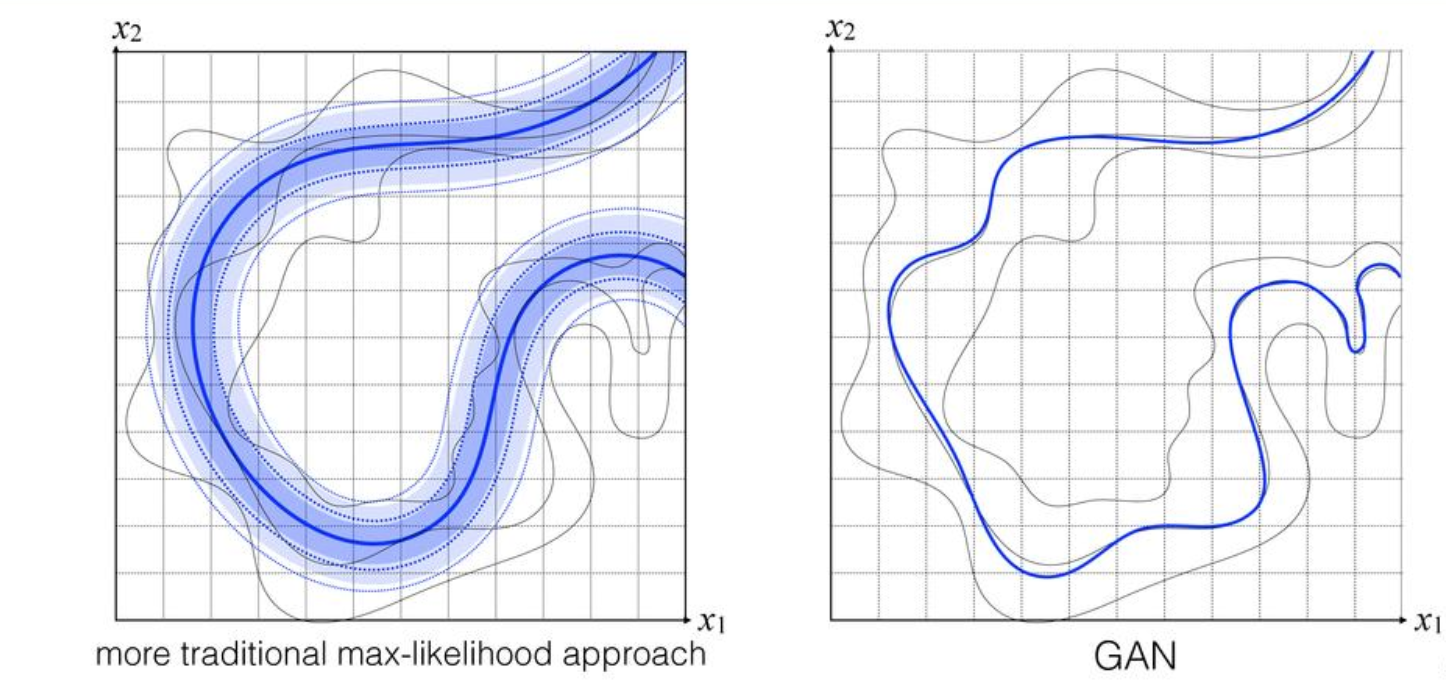
\includegraphics[width=\textwidth]{images/ml_vs_gan.png}
\caption{MLE против неявных вероятностных моделей~\cite{vetrovgan}}
\label{ml_vs_gan}
\end{figure}

\subsubsection{Дискретные данные}
Тонкое место GAN для дискретных значений - вторая компонента в 
Формуле~\ref{gan_opt}. А именно, нам надо уметь "пробросить" градиент через 
$D(G(z))$ по весам генератора. Это значит, что генератор не может производить
дискретных данных. Устранение такого ограничения - важное направление в GAN
в частности и в генеративных моделях в целом. 
Следуя \cite{1701.00160}, есть как минимум 3 очевидных пути обойти эту проблему:
\begin{itemize}
    \item Алгоритм REINFORCE~\cite{reinforce} из обучения с подкреплением
    \item Дифференцируемые методы сэмплирования из дискретного распределения~\cite{1611.00712, 1611.01144}
    \item Переход в непрерывное пространство, подразумевающее возможность 
    обратного декодирования (то есть, мы предсказываем вектор, а по ниму нужное
    слово)
\end{itemize}
Эти подходы нашли свои отражения в конкретных 
реализациях~\cite{seqgan, leakgan, gsgan}.

\section{Данные}
В этой главе происходит описание используемых данных.

Для тестирования работоспособности тех или иных подходов, нам потребуются 
текстовые данные, каждый сэмпл которых представляет из себя цельный отрывок
длиной в пару предложений. Одна из основных задач - преодолеть ограничение в 
длине генерируемых примеров ($10$-$15$ у разных статей~\cite{text_vae}), 
продолжая поддерживать связность. Мы же условимся расширить длину в два раза, до 
$30$ слов. Для простоты, мы возьмем возьмем категориальное бинарное свойство 
окраски текста. Чтобы увеличить датасет, мы также не будем требовать полной 
разметки.

Для размеченной части хорошо подходит Стэнфордский датасет (SST) для анализа 
эмоциональной окраски, основанный на базе данных отзывов о фильмах~\cite{sst}.
Чтобы сохранить область и форму данных, неразмеченная часть также была взята
из отзывов фильмов, но уже из набора данных IMDB~\cite{imdb}. Также, мы считали 
примерами без разметки часть данных SST, которая имела нейтральную окраску. Мы 
обрезали сэмплы с префиксам, длиннее $30$ символов, по границам предложений, 
чтобы выровнять длину.
Итого, мы получаем около $30000$ сэмплов для обучения и по $3000$ для валидации 
и тестирования. Для полного сравнения со статьями~\cite{text_vae, text_cvae}, 
мы также протестируем работу на данных только из SST и будем использовать 
похожий подход для тестирования классификатора.

Сырые входные данные также нуждаются в предобработке. Для токенизации, лучше 
всего при тестировании показал себя BPE encoding~\cite{wiki:bpe}. Его 
преимущество также в том, что он никак не зависит от конкретного языка, поэтому 
данное решение будет подходить и для других данных. Следуя примерам других 
статей~\cite{text_vae}, мы ограничимся наперед заданным ограничением на размер 
словаря - $15000$. Это также необходимо, чтобы избежать резкого увеличения 
количества весов при полносвязном слое перед софтмакс активацией (как несложно 
понять, здесь наблюдается квадратичный рост). Словарь будут также дополнять $4$ 
служебных слова - $\bos$, $\eos$, $\unk$ и $\pad$ - символы начала и конца, 
обрамляющие любой входной пример, а также символ пустоты при отступе символ
отсутствующего слова.

Мы будем объединять примеры в батч фиксированного размера, один к одному. 
Естественным образом, разные примеры имеют разную длину, поэтому недостающие
элементы заполняются символом $\pad$. Здесь мы также применим одну и популярных 
оптимизаций - объединять примеры в батч можно примерно одинакового размера, 
тогда и не придется заполнять половину всего тензора условным символом, так как 
длина всего батча равна максимальной длине примеров в нем.

Мы не делаем никаких строгих предположений о структуре данных, 
кроме последовательности из дискретных значений. 
Таким образом, в дальнейшей работе построенная модель может быть использована 
для генеративных задачах в другой области.

\section{Оценка качества}
Данная глава посвящена способам оценки алгоритмов генерации, а также тому, как 
правильно представить и сравнить результаты работы генеративных моделей.

Лучший и самый надежный способ оценить качество генерации - автоматические 
метрики и воспроизводимое окружение. К сожалению, большинство стандартных метрик
обладает некоторым количеством недостатков. Они могут либо плохо коррелировать
с человеческим восприятием, либо требовать много вычислительных 
ресурсов, а также быть зависимыми от конкретного приложения. Поэтому, все еще 
остра необходимость в метрике для генеративных задач, которую можно было бы 
использовать в любом окружении, не затрачивая много ресурсов~\cite{book:salp}.
Мы же опишем лучше всего подходящие к нашей задачи метрики, 
их преимущества и недостатки.

\subsection{Perplexity}
Perplexity используется для оценки того, насколько данная последовательность 
вероятна для текущей модели. Мы хотим присваивать большую вероятность 
предложениям, имеющий больший смысл и правильную грамматическую структуру. 
Эта величина которая будет отвечать за правдоподобность генерируемых примеров. 
Perplexity довольно часть используется в статьях по языковым моделям и машинному 
переводу, поэтому ее значения удобно соотносить и 
сравнивать с уже имеющимися результатами.

Процесс оценки следующий: мы разбиваем данные на тренировочную и тестовую 
выборки, используя для обучения только тренировочную часть. После оцениваем,
насколько вероятны данные из тестовой выборки, усредняя результат по всем 
примерам. Далее, такие оценки могут быть использованы для сравнения различных 
моделей и подходов к генерации~\cite{lecture:lm}.

Чтобы посчитать Perplexity используется Формула~\ref{perplexity}. Интуитивно,
это величина, обратная совместной вероятности слов в предложении. То есть, 
минимизация Perplexity эквивалентна максимизации совместной вероятности, поэтому
нас будут интересовать понижение значения Perplexity. Совместная вероятность 
удобно раскладывается в последовательное произведение вероятностей слов 
(Формула~\ref{perplexity_exp}) по цепному правилу.

\begin{equation}
\label{perplexity}
PPL(w) = P(w_1, \cdots, w_{|w|}) ^ {-\frac{1}{|w|}}
\end{equation}

\begin{equation}
\label{perplexity_exp}
P(w_1, \cdots, w_{|w|}) ^ {-\frac{1}{|w|}} = \sqrt[|w|]{\frac{1}{P(w)}} = 
\sqrt[|w|]{\frac{1}{\prod^{|w|}_{i=1}{P(w_i | w_{<i})}}}
\end{equation}

Основная сложность подсчета заключается в оценки совместной вероятности $P(w)$.
Более ранние работы из подходов, основанных на статистике, предлагали оценку, 
основанную на $N$-граммных методах (Формула~\ref{perplexity_ngram}). 
Эффективность такого подхода растет с ростом $N$ (Таблица~\ref{ngram_comp}), 
но он требует большого количества времени, которое также растет, на подсчет 
количества $N$-грамм $Count(w)$. 
Поэтому, такой подход к оценке вероятности не позволит быстро и хорошо оценить 
эффективность модели.

\begin{equation}
\label{perplexity_ngram}
P(w_i | w_{<i}) \approx P(w_i | w_{<i-N+1}) 
\approx \frac{Count(w_i, \cdots, w_{i-N+1})}{Count(w_{i-1}, \cdots, w_{i-N+1})}
\end{equation}

\begin{table}[H]
\centering
\begin{tabular}{c | c c c}
\toprule
Тип & Униграммы & Биграммы & Триграммы \\
\midrule
Perplexity & 962 & 170 & 109 \\
\bottomrule
\end{tabular}
\caption{Сравнение Perplexity для N-граммных методов~\cite{book:salp}}
\label{ngram_comp}
\end{table}

Заметим, однако, что для совместной вероятности нам всего лишь нужно уметь 
считать вероятность следующего слово по контексту-префиксу из предшествующих 
ему. Явный доступ с такому распределению позволяют получить модели с 
генератором - рекуррентной нейронной сетью, например, основанные на RNN и VAE. 
На очередном шаге RNN мы можем после оценить вероятность следующего слова, 
выбрав нужную компоненту после софтмакс активации.

Сложность, возникающая в процессе подсчета Perplexity, состоит в том, что 
некоторые части предложения, оцениваемые моделью, склонные получать очень 
низкую вероятность, ввиду своей нечастой встречаемости или отсутствия в 
словаре, построенном на тренировочном множестве. Примером могут послужить редкие 
имена собственные или стилистические особенности. В результате Perplexity, 
подсчитанная на таких примерах, стремится к $\infty$, переставая быть 
репрезентативным значением. Так как нам интересна эффективность работы "в 
среднем", без рассмотрения частных случаем с редкими словами, мы можем заменить 
такие плохие значения Perplexity константным большим числом (конкретное 
значение варьируется и зависит от задачи). Еще один минус Perplexity связан с
численным подсчетом: мы либо будем считать произведение вероятностей, либо 
сумму дорогостоящих операций $\log$ при переходе в $\log$-пространство.

\subsection{BLEU}
BLEU~\cite{bleu} это алгоритм для оценки качества машинного перевода из одного 
естественного языка на другой. 
Основная идея BLEU - чем ближе машинный перевод к эталонному
человеческому, тем лучше. BLEU до сих пор остается самой популярной и низкой
по стоимости метрикой, использующуюся повсеместно в задачах, связанных с 
генерацией текста.

Несмотря на свои недостатки~\cite{bleu_critique}, BLEU позиционируется как 
метрика имеющая высокую корреляцию с человеческим пониманием качества. По 
крайней мере, до сих пор не было предложено метрики, превосходящей BLEU по 
качеству оценки перевода. В последнее время, принимаются попытки расширить 
определение BLEU или даже переделать алгоритм в набор дифференцируемых
преобразований, так, чтобы метрику напрямую можно было бы оптимизировать в 
процессе обучения, но такие подходы до сих пор не пользуются большой 
популярностью.

BLEU используется как метрика, оценивающая качество перевода целого корпуса 
текста и теряет значимость, если с помощью нее пытаются оценить одно или
несколько предложений. BLEU - это число в промежутке от $0$ до $1$. Для 
одного примера, данная метрика считается по кандидатам, которых выдала модель 
и нескольким эталонным вариантам перевода (одна и та же фраза может иметь 
несколько популярных или общепринятых способов быть переведенной). 
Варианты перевода получаются, если модели присваивает большую вероятность сразу 
нескольким кандидатам. 
Эталонные варианты обычно получаются от разных профессиональных переводчиков, 
чтобы результаты были декоррелированы и система оценки была более устойчивой 
(Рис.~\ref{bleu_example}). Это также позволяет бороться с проблемой
полноты в оценке.

\begin{figure}[H]
\centering
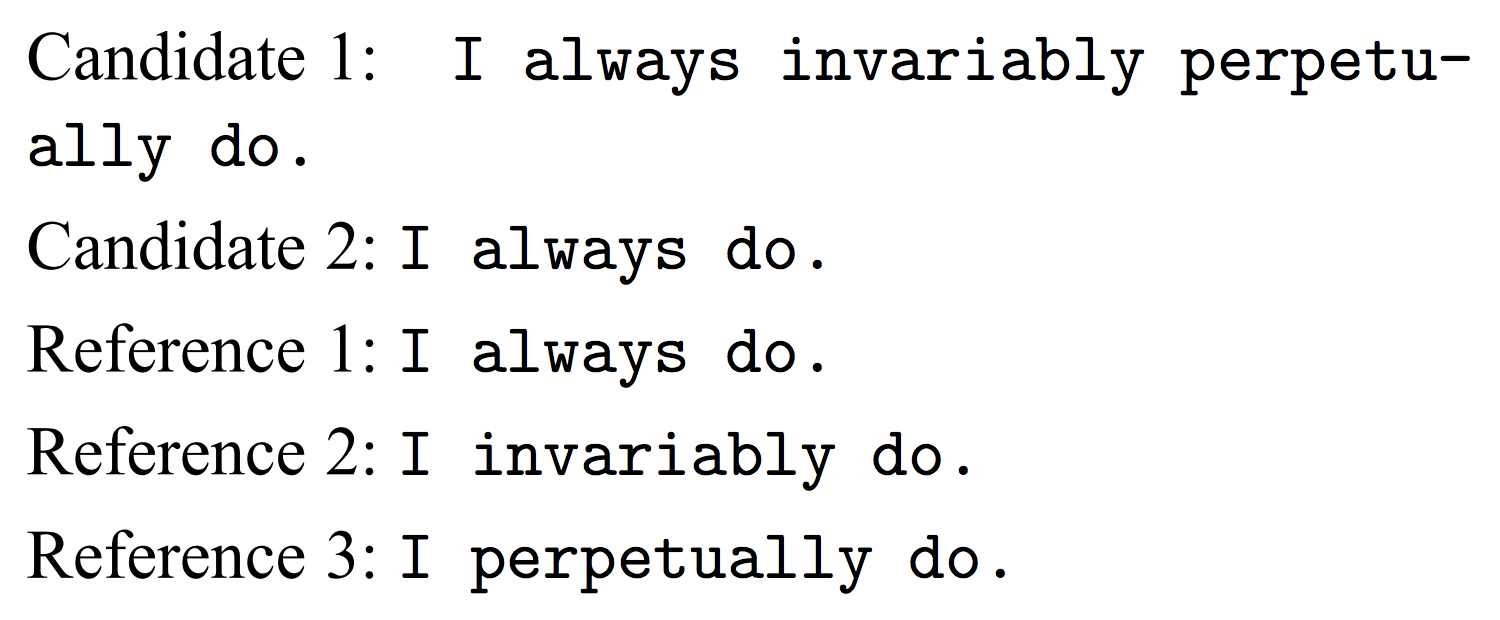
\includegraphics[width=0.6\textwidth]{images/bleu_example.png}
\caption{Пример для подсчета BLEU}
\label{bleu_example}
\end{figure}

BLEU - метрика, основанная на $N$-граммной схожести предложений. Для каждого $n$
мы считаем точность $p_n$ по Формуле~\ref{bleu_pn}. $Count(ngram)$ - это 
количество вхождений конкретной $ngram$-мы во все эталонные примеры. 
$Count_{clip}$ считается по Формуле~$\ref{bleu_countclip}$. Фактически, $p_n$
показывает точность вхождений $n$-грамм из кандидатов в эталоны.

\begin{equation}
\label{bleu_pn}
p_n = \frac{\sum\limits_{C \in \{candidates\}}{\sum\limits_{ngram \in C}{Count_{clip}(ngram)}}}{\sum\limits_{C' \in \{candidates\}}{\sum\limits_{ngram' \in C}{Count(ngram')}}}
\end{equation}

\begin{equation}
\label{bleu_countclip}
Count_{clip}(ngram) = min(Count(ngram), |\{references\}|)
\end{equation}

Далее, для подсчета BLEU мы берем геометрическое среднее $p_n$ с весами, 
суммирующимися до единицы, умножая результат на "штраф за длину" 
(brevity penalty, BP). Мы берем $n$-граммы, начиная с униграмм вплоть до $N$, 
где $N$ обычно равняется $4$ или $5$. BP вычисляется по Формуле~\ref{bleu_bp}. 
$c$ - это сумма длин кандидатов, $r$ - сумма длин ближайший по длине эталонов 
по каждому кандидату (такая логика нужна, чтобы не штрафовать коротких 
кандидатов слишком сильно). Итоговое значение BLEU считается по 
Формуле~\ref{bleu_final}. 
Взяв логарифм, получаем удобную к вычислению и последующему
сравнению Формулу~\ref{bleu_final_log}. Стоит также отметить, что стандартные 
веса в формуле BLEU распределены равномерно, т.е. $w_n = \frac{1}{N}$.

\begin{equation}
\label{bleu_bp}
BP = 
\begin{cases}
1 &\text{if } c > r\\
e^{1 - \frac{r}{c}} &\text{if } c \leqslant r
\end{cases}
\end{equation}

\begin{equation}
\label{bleu_final}
BLEU = BP \cdot exp(\sum^{N}_{i=1}{w_n \log{p_n}})
\end{equation}

\begin{equation}
\label{bleu_final_log}
log BLEU = min(1 - \frac{r}{c}, 0) + \sum^{N}_{i=1}{w_n \log{p_n}}
\end{equation}

Так как BLEU основана на $N$-граммной схожести предложения, она может подойти
не только для оценки качества перевода, но и для оценки качества генерации: в 
качестве кандидата теперь будет выступать сгенерированный сэмпл, а
в качестве эталонов - набор из валидационного множества, не встречаемого при
обучении. Далее, такое значение мы усредняем по нескольким примерам для 
устойчивости.

Данный подход обладает рядом недостатков: недостаточно хорошая корреляция с 
человеческой оценкой, большая дисперсия и невозможность сравнения с другими 
задачами, использующими BLEU как основную метрику (из-за другого использования). 
Однако, есть и преимущества: независимость от окружения, 
отсутствие предположений о внутренней структуре модели 
(в отличии от Perplexity), низкая стоимость подсчета и отсутствие проблем с
редкими словами.

Данная метрика будет основной в данной работе и отвечает за правдоподобие 
сгенерированных примеров. Отчасти это связано с невозможность обойти проблемы
Perplexity, отчасти с доступностью сравнений с результатами из других статей.

\subsection{Self-BLEU}
Заметим, однако, что не всегда большой BLEU свидетельствует от хорошей работе
генеративной модели. Рассмотрим крайний случай: $\pmodel$ является вырожденным
распределением, дающим $100\%$ вероятности одному хорошему примеру. BLEU метрика
высокая, однако результат далек от идеального. Таким образом, помимо 
правдоподобия, нам также необходимо поддерживать разнообразие генерируемых 
примеров. Это одно из важные свойств хорошей генеративной модели, которому
часто не придают большого значения.

Для того, чтобы подсчитать разнообразие примеров, можно применить один из 
несложных способов - простое расширение BLEU, основанное на подсчете метрики на 
сэмплах с самими собой. 
Мы условимся называть эту метрику Self-BLEU. Self-BLEU это усредненное BLEU по 
каждому из примеров со всеми остальными. Условно её можно описать 
Формулой~\ref{self_bleu}.

\begin{equation}
\label{self_bleu}
SELF\_BLEU(S) = \frac{1}{|S|} \sum\limits^{|S|}_{i=1}{BLEU(\{S_i\}, S \setminus \{S_i\})}
\end{equation}

Self-BLEU обладает таким же набором недостатков и преимуществ, но гораздо менее
распространен, в следствии чего показания не получится сравнить с другими 
результатами. В отличии от BLEU, нас будут интересовать низкие значения 
Self-BLEU, так как нам интересно более полно моделировать $\pdata$, не 
ограничиваясь небольшим количеством хороших сэмплов.

\subsection{Человеческая оценка}
Пожалуй, лучший способ оценить качество генеративных моделей - человеческая 
оценка.
В отличии от некоторых задач машинного обучения, в генерации мнение и 
способности человека - абсолют. Нам незачем создавать новые экземпляры текста, 
если они не могут быть правильно проинтерпретированы и поняты человеком. 
Поэтому, человеческое восприятие - важный компонент в генеративных моделях. 
Проблемы такого подхода - контекст (культурный, социальный, исторический), из-за
чего разные группы людей могут оценивать разные сэмплы по-разному и большая
стоимость оценки (с точки зрения ресурсов и времени).

Частично, справиться с последней проблемой помогают набирающие популярность 
сервисы, позволяющие размещать в Интернета задания, в том числе и задания по
разметке данных и оценке тех или иных данные по различным
критериям~\cite{yatoloka, mturk}. Все же, такие сервисы подходят скорее для 
промышленных задач, чем для научной работы, требуя значительных средств для 
хорошего качества. Так или иначе, чтобы получить устойчивую оценку, нам 
понадобится выдавать одно и тоже задание на разметку разным людям, усредняя
общий результат, поэтому окупаемость такого подхода требует подробного 
рассмотрения.

Подходы с человеческой оценкой качества - частый способ оценки в задачах 
информационного поиска, но их также применяют и в задачах 
генерации~\cite{1606.03498}. В данной работе человеческая оценка 
использовалась разве что в качестве первой проверки (вырожденный результат 
виден невооруженным взглядом), ввиду недостатка ресурсов и большого времени на 
оценку. Тем не менее, такой подход может быть использован в дальнейшем.

\section{Решение}
В данной главе описаны наиболее удачные подходы, которые дали ощутимый прирост в 
качестве работы, и трудности, с которыми пришлось столкнуться в процессе 
реализации.

\subsection{Реализация}
За основу будущей модели было взято описание Contitional VAE~\cite{text_cvae}. 
Во-первых, такая модель эффективно умеет работать в 
условия данных с неполной разметкой. Во-вторых, она предоставляет механизм
условной генерации дискретных значений, позволяя явно задавать необходимые 
свойства. В-третьих, в самой статьи описаны удачные подходы для успешного 
обучения.

Модель была реализована на фреймворке PyTorch 0.4~\cite{pytorch} (для 
красивого, расширяемого и поддерживаемого кода). Код доступен в открытом 
репозитории~\cite{github}. При реализации особое внимание уделялось скорости 
обучения и генерации, так как это узкий момент в оригинальном алгоритме. 
Дело в том, что во время одной итерации
нужно уметь сэмплировать два разных батча из $x$ для прогона одного шага 
оптимизации. Так как сэмплирование происходит слово за словом, любая сложная 
логика на декодере оборачивается понижением производительности в несколько 
раз.

В качестве дискриминатора из оригинальной статьи была взята простая сетка без
нелинейных слоев, не учитывающая $N$-граммы. Такая модель показала низкий 
прирост качества классификации после обучения и не способна правильно 
классифицировать сложные длинные куски текста, в которых не раз может меняться
направление мысли, тон, настроение и эмоциональная окраска в целом.
Дискриминатор из оригинальной статьи был переписан на 
CNNEncoder~\cite{1510.03820}, представляющий из себя комбинацию из нескольких 
сверточных слоев, связанными max-pooling'ом и нелинейными активациями (SELU). 
Такая модель также учитывает $2$-$3$-$4$-$5$-граммы слов, показывая хороших 
результаты на бинарной классификации предложений. Один из очевидных плюсов 
такого дискриминатора - отсутствие полносвязных и рекуррентных слоев, из-за 
которых скорость обучения заметно падает.

В качестве векторного представления для слов был взят набор предобученных
векторов GLoVE размерностью $100$. Веса не замораживались во время обучения,
так как, фактически, мы брали данные из конкретной области - отзывов о фильмах,
поэтому и контекст использования может слегка сместиться. В то же время, данных
для обучения было достаточно, чтобы не потерять способность к обобщению.

Авторы оригинальной Text VAE~\cite{text_vae} использовали несколько трюков, 
позволяющих эффективней обучить модель на текстовых данных, которые также были 
применены и здесь. Во-первых, помимо обычного рекуррентного 
дропаута~\cite{wiki:dropout} между слоями и шагами в RNN, был применен 
WordDropout - небольшой расширение, позволяющее реже смотреть на последнее 
слово при выводе и генерации. Это легко обобщается до KWordDropout - аннулируем
$k$ последних слов с вероятностью, распределенной по убывающей от конца 
функцией. Интуиция тут примерно следующая: чем длиннее текст, тем вероятнее 
последнее словосочетание, а не единичное слово, повлияют на выбор следующего. 
Вероятность для дропаута была взята со значением $0.3$, повторяя выбор 
оригинальной статьи. Во-вторых, вес переменный kl-терма был заменен с 
линейного роста на рост по гладкой $\tanh$, переведенной в $[0, 1]$. Это 
позволило немного улучшить оптимизацию kl-части, введя более гладкий переход 
при обучении.

Следуя~\cite{fastai}, мы использовали метод обучения 
SGDR~\cite{1608.03983}, основанный на Adam с $3$ рестартами. Мы обрезали 
градиент, для предотвращения взрывов на начальной стадии обучения со значением
$10$. Скорость обучения бралась традиционна маленькой для подобных задач, 
изменявшись в цикле с $1e-2$ до $1e-3$. Размер батча - $64$. Все обучение, как 
и генерация, происходило на графическом процессоре GeForce GTX $1080$, что
заметно ускоряло процесс подбора параметров.

Большинство значений подобрано эмпирически на валидации или 
взято из оригинальной статьи, а некоторые вещи удалось видоизменить или 
обобщить для большей устойчивости к длине генерации.

\subsection{SRU}
Как уже было сказано выше, для повышения скорости обучения и сэмплирования 
важно иметь быстрые энкодер и генератор. Одна итерация в цикле оптимизации, 
эквивалентному Wake-Sleep алгоритму~\cite{text_cvae}, требует сэмплирования двух
батчей данных $x$, один из которых параметризован конкретным свойством $c$.
Процесс генерации - самый трудозатратный во всем алгоритме, во многом из-за
реализации его в виде алгоритма Beam Search, требующего поддержания $k$ 
кандидатов на каждый пример из батча. Наивная реализация показала, что 
одна полная оптимизация модели может занимать десятки часов, что 
катастрофически много для тестирования, подбора параметров и архитектурных 
выборов. Итак, решено было ускорить процесс за счет двух оптимизация: замены 
RNN на CNN и переписывании алгоритма генерации в виде векторных операций на 
графическом процессоре.

SRU~\cite{1709.02755} - идеологически, рекуррентная нейронная сеть, в которой
матричные операции внутри очередного шага заменены на сверточные нейронные
слои. Для использования в данной модели была заимствовано, доделана и
изменена референсная реализация SRU. Такая вариация RNN позволяет минимум
вдвое сократить время на обучение, вдвое же увеличив количество слоев.
Результаты показывают, что $6$-слойные SRU с дропаутом при долгой оптимизации
могут даже увеличить результаты в метрики терминах $Perplexity$. Таким
образом, замена RNN в энкодере и генераторе на SRU даст ощутимый прирост в
скорости и эффективности. Однако, следует учесть, что обучение генератора с
SRU теряется информативность скрытых векторов, поэтому строить механизм
внимания (attention), основываясь на их связи, не получается. Внимание играет
важную роль в построение интерпретируемой модели с увеличенной длиной генерации,
поэтому решено было реализовать $3$-слойный SRU без дропаута
(чтобы помочь энкодеру, особенно на начальном этапе)
в качестве энкодера, и $2$-слойный GRU с дропаутом в $0.3$ в качестве
генератора.

Суммарно, обе оптимизации дали почти шестикратный прирост в скорости,
что позволило сократить до часа с небольшим процесс обучения до сходимости.

\subsection{Стохастический Beam Search}
Выше, уже было сказано о дихотомии двух подходов к генерации. С одной стороны,
мы можем всякий раз сэмплировать очередное новое слово и двигаться дальше. С
другой стороны, мы можем детерминировано выбирать $\argmax$. Оба подхода 
обладают рядом недостатков: с одной стороны мы заботимся о разнообразии, с 
другой - о высокой совместной вероятности у кандидатов, т.е. правдоподобии.
Более того, случай с $\argmax$ - вырожденный, мы всегда будем ровно один
уникальный сэмпл при генерации. Необходимо придумать компромисс, с помощью 
которого можно эффективно получать длинные сэмплы.

Интуитивно, мы хотим просэмплировать префикс, задав основную часть выражения и 
добрать суффикс с $\argmax$. Вариация алгоритма beam search, которая позволяет
найти удачный компромисс для двух подходов, приблизив нас к интуиции - 
стохастический beam search~\cite{sbeamsearch}. Мы также поддерживаем $k$ 
кандидатов, но новых выбираем не через максимизацию, а через честное 
сэмплирование. Параметр $k$, подбираемый на валидации, позволяет эффективно 
найти нечто среднее между двумя крайними случаями. Помимо этого, алгоритм 
также параметризуется температурой софтмакс активации, чтобы напрямую 
контролировать разнообразие. Итого, получаем гибкий алгоритм с реализацией в 
векторных операциях на графическом процессоре, через который можно выразить 
все остальные подходы, контролируя $k$ и температуру $\tau$. Например, greedy 
decoding (жадный алгоритм) выражается через $k=1$ и $\tau=\epsilon > 0$ 
(распределение стремится к one-hot). 
Параметр, подобранный при запусках: $k=3$, $\tau=1$ не изменялось 
во время обучения, но её увеличение дает эффективный способ повышения 
разнообразия.

\subsection{Self-Attention}
Основной механизм увеличения длинны генерации в стандартных seq2seq моделях
для машинного перевода - использования механизма внимания (attention). 
Фактически, на каждом шаге мы добавляем информацию о коррелируемости всех 
предыдущих шагов с энкодера, что позволяет учитывать даже долгосрочные
зависимости между словами в предложении. Такое расширение не только позволяет
сохранять связность, но и добавляет модели интерпретируемости: теперь мы можем
нарисовать матрицу внимания, которая покажет зависимости слов от контекста до 
них (Рис.~\ref{attention}). Такая матрица внимания существует для каждого 
кандидата при генерации.

\begin{figure}[H]
\centering
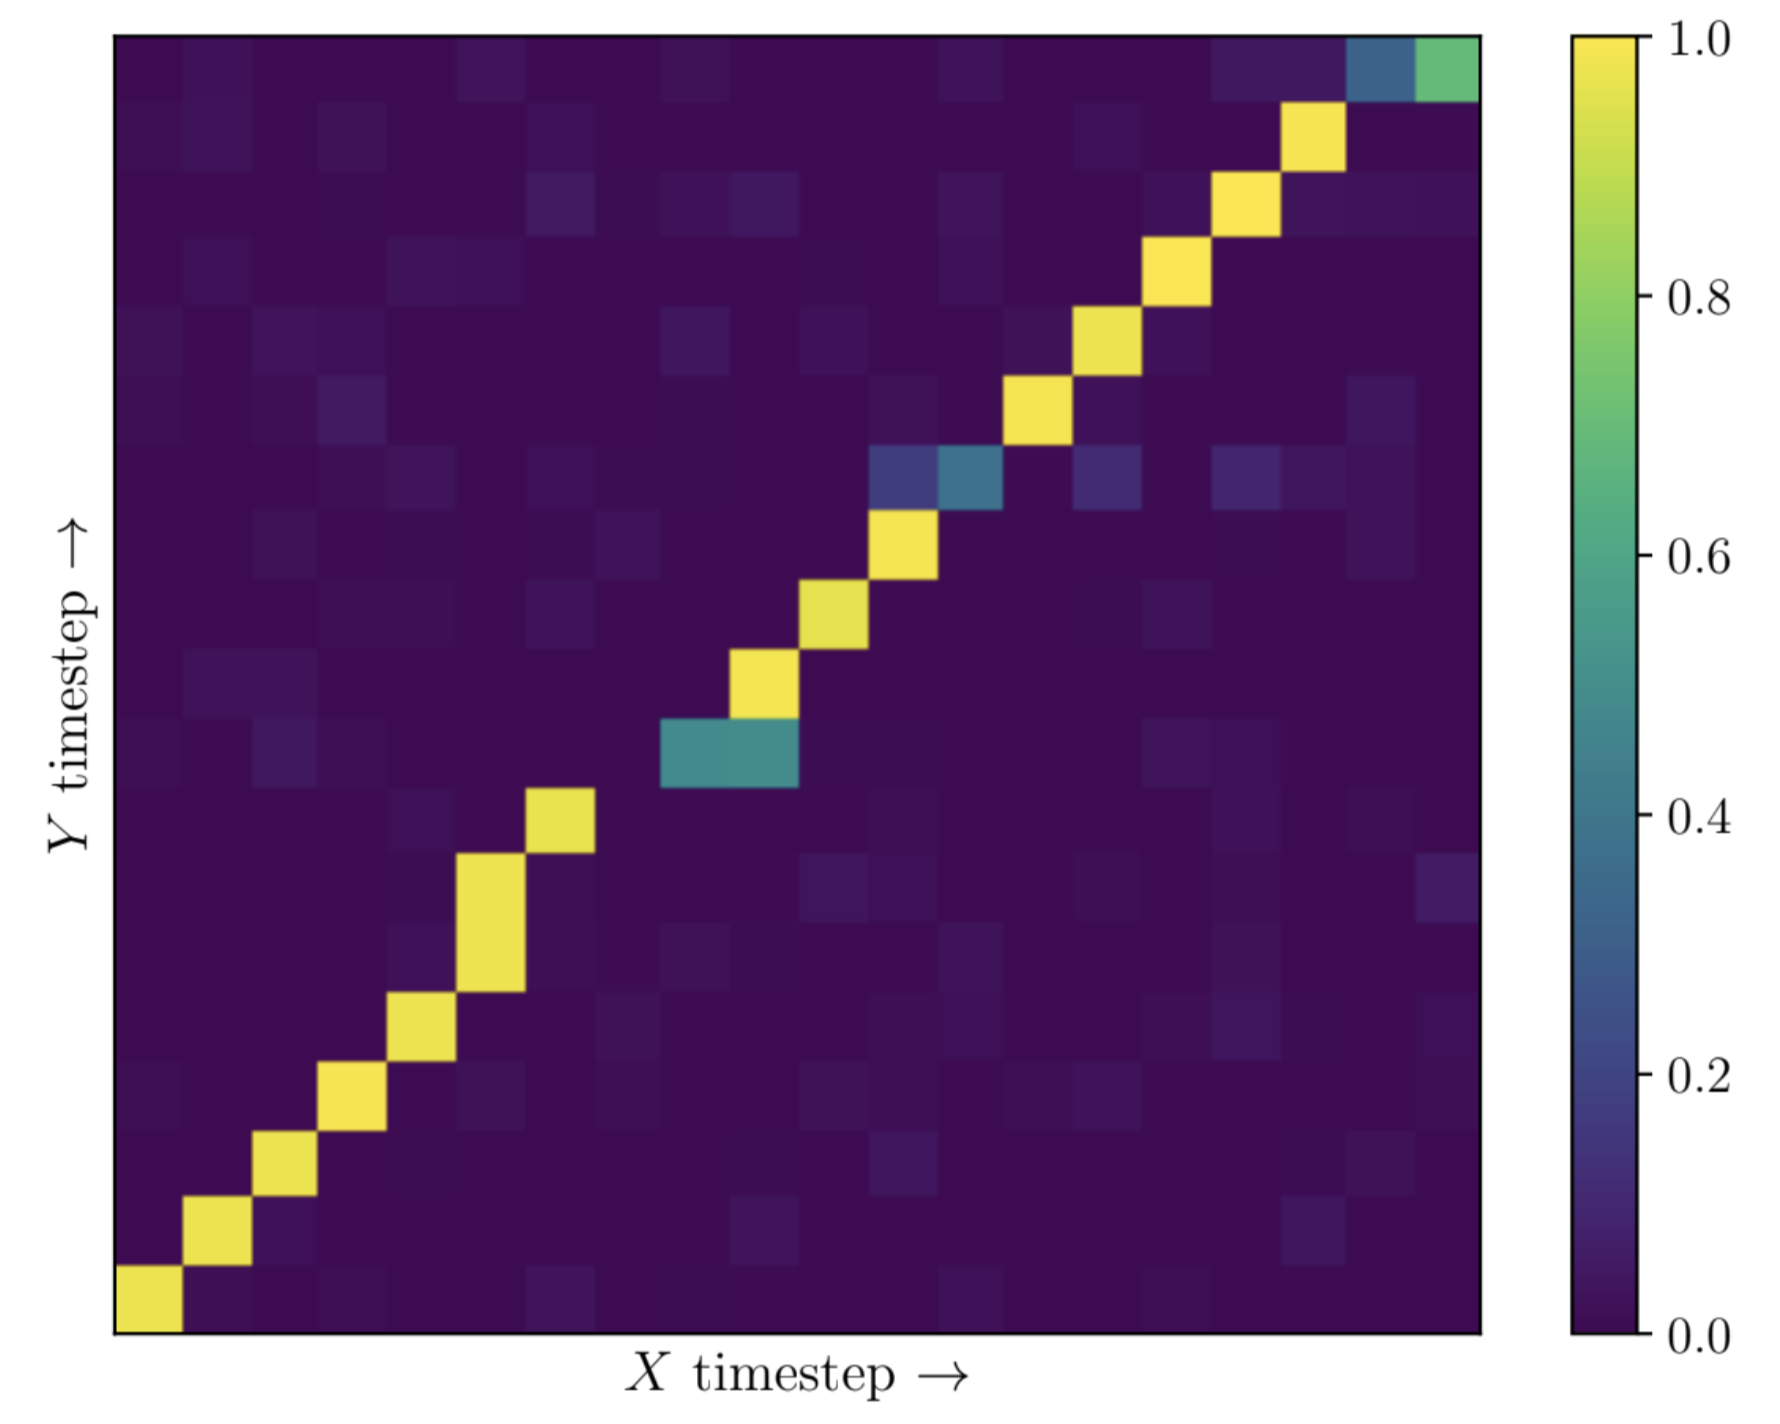
\includegraphics[width=0.8\textwidth]{images/attention.png}
\caption{Матрица внимания}
\label{attention}
\end{figure}

Проблема с генеративными моделями заключается, однако, в отсутствии энкодера 
(точнее, отсутствии доступа к нему во время генерации). Мы предлагаем 
расширение механизма внимания на генеративные модели: механизм 
самовнимания (self-attention). Похожие по идеологии подходы стали популярны в 
совсем недавних статьях, поэтому и предложено схожее 
название~\cite{1706.03762, 1805.08318}. Фактически, мы используем 
информацию с предыдущих шагов декодера, добавляя ее на очередном шаге при 
выводе (Рис.~\ref{self_attention}). Важный момент - как считать матрицу 
внимания, чтобы правильно учесть последнее слово. Для этого, при определении 
коррелируемости использовались новый $o'_i$, представляющий сбор информации с 
предыдущих шагов, и старые $o_i$. Для реализации 
была выбрана вариация общего (general) внимания с полносвязными слоями до и 
после сбора векторов контекста с SELU-активацией после. Реализация была 
выполнена в виде отдельной сети-модуля для PyTorch, поэтому также может быть
использована в других моделях и задачах.

\begin{figure}[H]
\centering
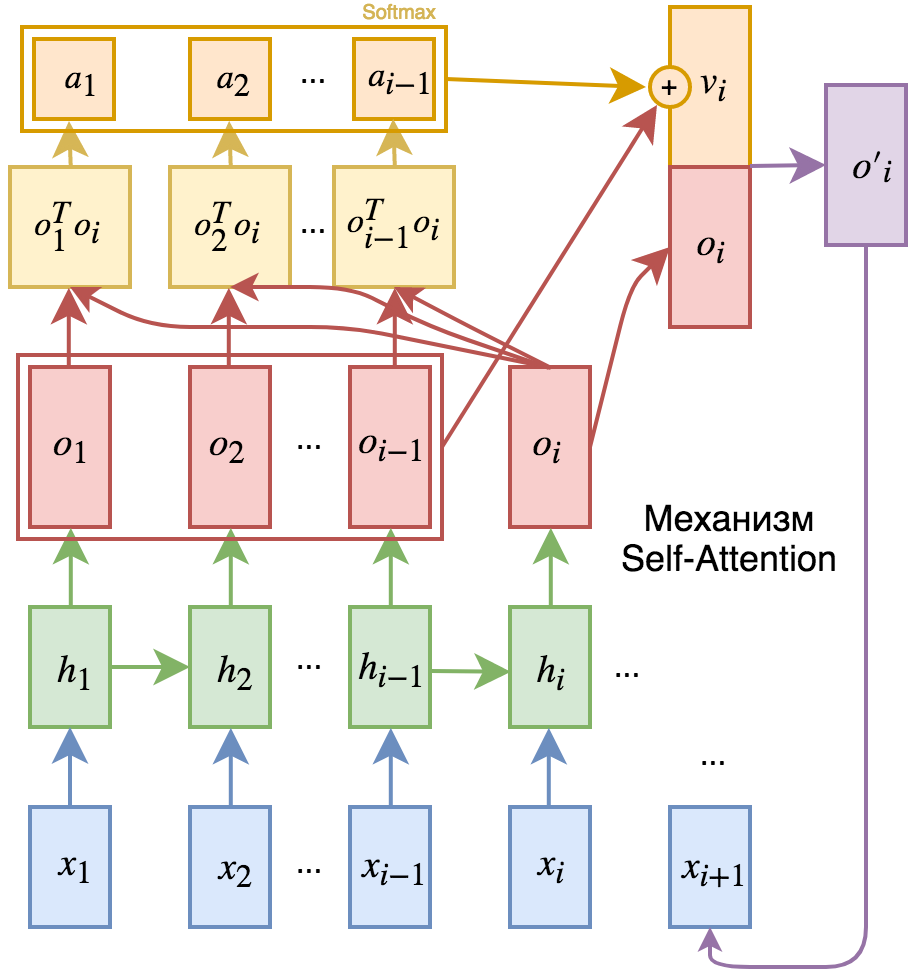
\includegraphics[width=0.7\textwidth]{images/self_attention.png}
\caption{Архитектура Self-Attention}
\label{self_attention}
\end{figure}

Важное преимущество, которое мы получили, реализовав данный механизм - резкое
повышение интерпретируемости (Рис.~\ref{sa_sample1}, \ref{sa_sample2}). На 
графиках изображены матрица внимания собранные при генерации конкретных сэмплов
. В генерации, мы движемся по оси $x$ слева направо и не можем смотреть в 
будущее, поэтому все веса находятся ниже транспонированной главной диагонали. 
Теперь явным образом наблюдаются не только зависимости одних слов и выражений 
от других, но и разнообразные вырожденные случаи (хотя они и будут видны 
невооруженным глазом в виде повторяющего партерна на матрице, все же позволяют 
обратить внимание на возможные проблемы в реализации и обучении). В общем и 
целом, такой механизм не только дал наибольший прирост на метриках, но и 
значительно расширил представление о том, как именно нейросеть генерирует
очередной сэмпл.

\begin{figure}[H]
\centering
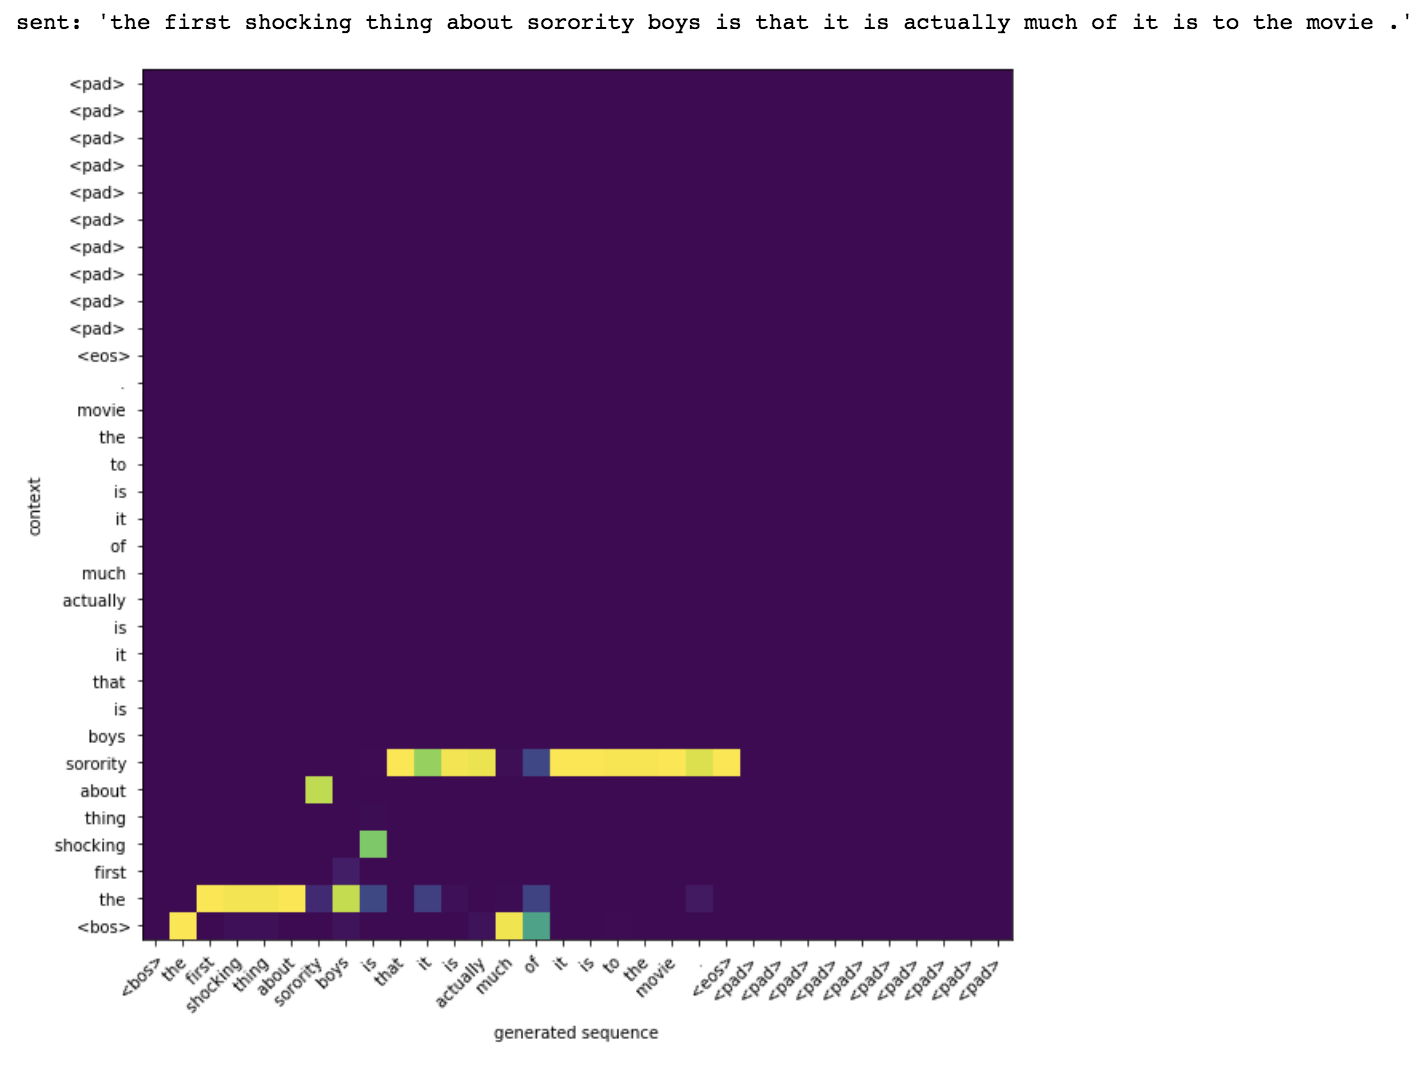
\includegraphics[width=\textwidth]{images/sa_sample1.png}
\caption{Матрица Self-Attention для конкретного кандидата 1}
\label{sa_sample1}
\end{figure}

\begin{figure}[H]
\centering
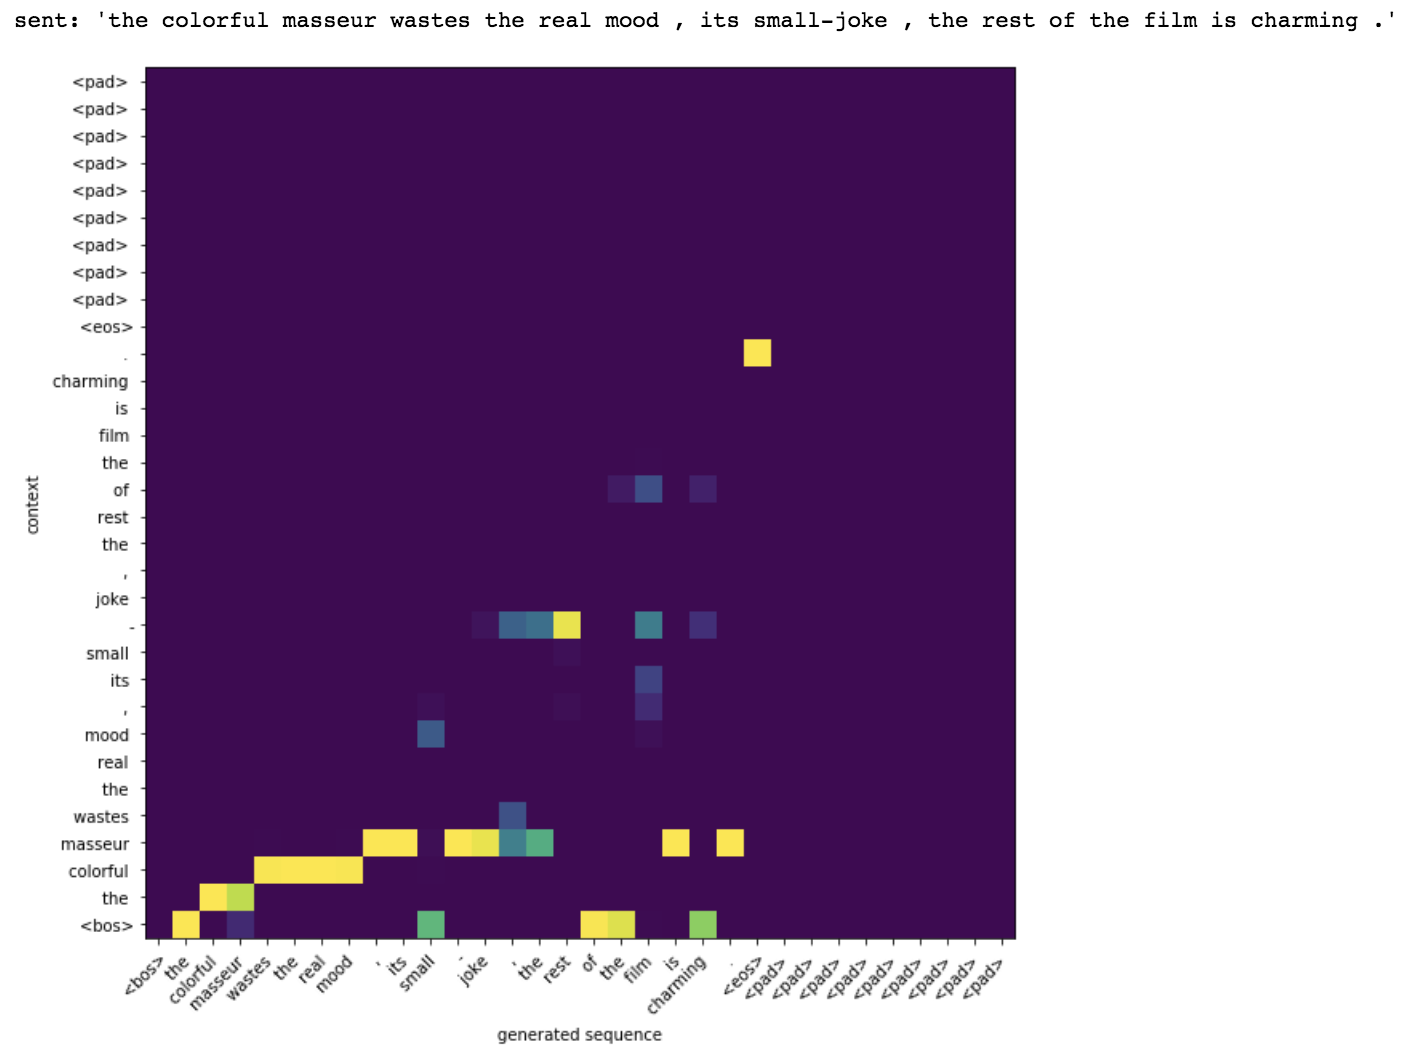
\includegraphics[width=\textwidth]{images/sa_sample2.png}
\caption{Матрица Self-Attention для конкретного кандидата 2}
\label{sa_sample2}
\end{figure}

\subsection{Штраф за покрытие на матрице внимания}
Еще один большой плюс матрицы внимания - возможность ввести регуляризацию на
кандидатов. Одной из самых больших проблем генерации является ранжирование 
кандидатов при beam search. Стандартный подход - ранжирование по логарифму 
совместной вероятности, т.е. произведению всех вероятностей на пути в дереве 
вывода (Рис.~\ref{beam_search}). Однако, как несложно понять, в таком случае 
более короткие примеры будут иметь больший шанс быть выбранными, просто потому 
что они заканчиваются раньше и не имеют добавки в виде префикса-вероятности, 
снижающем общую вероятность кандидата. 

Есть несколько способов избежать этого. Можно нормализовать вероятность по 
длине, можно добавить к очкам кандидата регуляризацию по длине 
$\beta \cdot |x|$. Однако, они плохо обощаются на вырожденные случаи с 
повторяемыми кусами текста. Следуя~\cite{1703.03906}, мы предлагаем подход в 
виде штрафа на матрице self-attention (Формула~\ref{coverage_penalty}). Такой
штраф добавляем к логарифму совместной вероятности для учета в итоговом 
ранжировании. Интуитивно, чем более заполнена матрица и чем более она 
соответствует случаю "каждое слово раздает единицу внимания всем другим", тем
лучше. Такой подход позволил чаще избежать вырожденных случаев
при генерации (слишком коротких, повторяющихся, незаконченных), увеличив 
итоговые метрики.

\begin{equation}
\label{coverage_penalty}
cp(A) = \sum\limits^{|x|}_{i=1}{\log \left[\min(\sum\limits^{|x|}_{j=1}{A_{ij}}, 1) \right]}
\end{equation}

\section{Результаты}
В данной главе проводится анализ результатов.

За базовую модель, основанную на принципе максимального правдоподобия 
(MLE), была взять обычная рекуррентная нейронная сеть на LSTM. Для 
тестирования на BLEU метриках будем использовать множества из 
$|X_{\texttt{gen}}|=500$ сэмплов.

Для подходов, основанных на генеративных состязательных сетях, были 
использованы референсные реализации с открытым исходным 
кодом~\cite{seqgan, leakgan, gsgan}.
GAN обладают
целым набором проблем при обучении, начиная от правильного сэмплирования 
латентного вектора для генератора, заканчивая расхождением в скорости обучения 
генератора и дискриминатора. Подходы, основанные на алгоритме 
REINFORCE (SeqGAN, LeakGAN), сходятся крайне медленно (до нескольких дней) 
из-за проблем с дисперсией, а некоторые реализации не заботились о 
воспроизводимости вычислений, поэтому использовать запустить их было 
проблематично. Результаты сравнения с $MLE$ представлены на 
Таблице~\ref{ganmle_table}.

\begin{table}[H]
\begin{tabular}{c | c c c c c c}
\toprule
Metrics & SeqGAN & MaliGAN & RankGAN & LeakGAN & TextGAN & MLE \\
\midrule
BLEU & 18.0 & 15.9 & 15.6 & \textbf{23.0} & 20.7 & 8.1 \\
Self-BLEU & 48.9 & 43.7 & 61.8 & 78.0 & 74.6 & \textbf{10.6} \\
\bottomrule
\end{tabular}
\caption{BLEU5 * $100$ для $500$ сгенерированных сэмплов}
\label{ganmle_table}
\end{table}

Столь высокие показатели BLEU метрик обусловлены в том числе и тем, что в 
генерируемого множестве часто попадаются одинаковые или почти одинаковые сэмплы, 
которые сопоставляются при подсчете $n$-грамм.
Видно, что несмотря на высокие показатели $BLUE$, все GAN проигрывают 
обычному принципу максимального правдоподобия в разнообразии. Фактически, это
означает, что GAN могут выдавать несколько хороших примеров, но не способны
поддерживать разнообразие генерации. Одна из возможных причин - традиционная 
проблема с правильным сэмплированием внутри алгоритма REINFORCE. Другая 
возможная причина связана с проблемой "mode collapsing"~\cite{mode_collapsing} 
- главной проблемой архитектуры генеративных конкурирующих сетей на данный 
момент (Рис.~\ref{ml_vs_gan}). 

Одно из заявленные свойств необходимого генератора - поддержание вариативности, 
которая тут намного оказалось хуже, чем у простой базовой модели. Поэтому, 
модели основанные на GAN в данный момент нуждаются в решении проблемы с 
разнообразием. Похожая проблема сейчас наблюдается и в случае непрерывных 
данных.

Результаты для предложенного расширения Conditional VAE представлены на 
Таблице~\ref{cvae_table}: 
\begin{itemize}
    \item $SBS_k$ - стохастический beam search, параметризованный $k$
    \item $CP$ - штраф на матрице внимания
    \item $SA$ - self-attention на генераторе
    \item $D_{ACC}$ - точность на классификаторе после генерации с заданным свойством
    \item $CVAE_{++}$ - CVAE плюс все удачные расширения, дополнения и изменения, описанные в главе "Решение"
\end{itemize}

\begin{table}[H]
\begin{tabular}{c | c c c c}
\toprule
Metrics & VAE & CVAE & $CVAE_{++}$ + SA & \textbf{$\boldsymbol{CVAE_{++}}$ + SA + CP + $\boldsymbol{SBS_3}$} \\
\midrule
$D_{ACC}$ & - & 83.483 & \textbf{84.263} & \textbf{84.263} \\
Perplexity & 150 & 104 & 84 & \textbf{83} \\
BLEU & 8.5 & 9.3 & 18.2 & \textbf{20.5} \\
Self-BLEU & 9.0 & 8.7 & 45.8 & \textbf{44.2} \\
\bottomrule
\end{tabular}
\caption{Метрики для CVAE}
\label{cvae_table}
\end{table}

Следуя~\cite{text_cvae}, точность на классификаторе $D_{ACC}$ проверялась уже 
после обучения на тестовом размеченном множестве. Видно, что с заменой 
дискриминатора, удалось сохранить и повысить высокую точность, не ухудшив 
остальные метрики.

Результаты Perplexity получились не слишком репрезентативными, оставаясь намного
позади лучших показателей в задачах языкового моделирования (это объясняется 
наличием регуляризацией на форму латентного пространства, помимо ошибки 
восстановления). Тем не менее, значения резко упали и при переходе к неполной
разметки и при использовании механизма внимания, что подтверждает их полезность.

Видно также, что резкий скачок в эффективности происходит при переходе к 
управляемой генерации (так мы можем использовать данные с неполной разметкой), а 
также при использовании механизма внимания. 
Стохастический beam search с регуляризацией
также добавляют прирост в метриках BLEU, что подтверждает их эффективность. При 
сравнении с Таблицей~\ref{ganmle_table} можно наблюдать общий эффект: при 
увеличении правдоподобия, разнообразие по Self-BLEU тоже значительно падает, 
но у расширенной версии CVAE оно остается на уровне лучших GAN, 
сохраняя при этом высокое правдоподобие.

Итак, предложенные оптимизации и расширения действительно смогли эффективно 
сохранить высокую правдоподобность и относительно хорошее разнообразие, при 
это увеличив длину генерируемых сэмплов вдвое. При этом, мы также эффективно 
расширили модель на условия с данными с частичной разметкой (которые чаще 
всего можно встретить в реальной жизни), сохранив при этом высокую точность 
классификации, а, следовательно, возможность эффективно параметризовать 
генератор требуемыми свойствами.

\section*{Заключение}
Современное глубокое обучение основано на способности вычислительных графов
быть дифференцируемыми. При переходе к дискретным значениям старые подходы
перестают работать, поэтому приходиться строить отображения дискретного 
пространства в непрерывное, что так или иначе ведет к проблемам с оптимизацией.
Задача генерации текста усложняется еще и тем, что 
при увеличении длины входных последовательностей быстро растет сложность по 
поддержанию связности, правдоподобия и разнообразия генерируемых сэмплов.

Современные генеративные модели все еще обладают рядом фундаментальных проблем,
которые не позволяют считать задачу генерации решенной. Ценность этой работы 
заключается не только в предложенном и описанном подходе, решавшем 
поставленную задачу, но и в трудностях, возникших при реализации и  
тестировании, указывающих на глобальные проблемы и очерчивающих границы 
применимости того или иного метода или модели.

В рамках данной работы можно выделить следующие основные результаты:
\begin{itemize}
    \item Удалось проанализировать текущие подходы к генерации текста, подробно изучены принципы и особенности работы генеративных моделей с дискретными значениями, намечены основные сложности и проблемы.
    \item Придуманы и описаны метрики для комплексной оценки качества генерации.
    \item Придуманы и реализованы способы, позволяющие справляться с существующими проблемами. Основная цель - увеличение длины генерируемых сэмплов, была успешно решена.
    \item Итоговая модель получилась не только эффективной в терминах метрик, но и интерпретируемой и гибкой. Свойство интерпретируемости, основанное на механизме внимания, не только поможет в дальнейшем правильно анализировать влияние того или иного изменения на результат генерации, но и правильно подбирать параметры при текущей реализации на новых данных.
\end{itemize}

Существует несколько вариантов для будущей работы:
\begin{itemize}
    \item Преодоление ограничения на выбор априорного и апостериорного распределения в моделях, основанных на VAE. Этого позволяют добиться модели, вбирающие в себя лучшие свойства VAE и GAN~\cite{vetrovgan, aae, alphagan}. Понадобиться исследовать возможность эффективного обучения данных моделей на дискретных данных.
    \item Запустить предложенную модель на дискретных не строковых данных. Например, на SMILES представлениях молекул, проанализировав процент валидных молекулярных структур, а также их разнообразие и получаемые свойства.
\end{itemize}

\bibliographystyle{ugost2008ls}
\bibliography{diploma.bib}

\end{document}
